
\section{Detailed \beetle{} BLiMP and MultiBLiMP results}

% Two-column layout of the Beetle main results table.
% Requires: \usepackage{booktabs,multirow,array}; \usepackage[table]{xcolor}
% Drops seed runs, method ablations (episodic/alibi/ewc/lamol/pre-pretrain),
% the B3 (0--100) variant, FW-24B runs, and the frontier-LLM baselines.
% Bold = per-language-pair column maximum.
\begin{table*}[t]
\centering\scriptsize
\setlength{\tabcolsep}{3pt}
\begin{minipage}[t]{0.49\linewidth}\centering
\begin{tabular}{ll l cc cc}
\toprule
& & & \multicolumn{2}{c}{\textbf{MultiBLiMP}} & \multicolumn{2}{c}{\textbf{MonoBLiMP}} \\
\cmidrule(lr){4-5}\cmidrule(lr){6-7}
\textbf{Pair} & \textbf{Data} & \textbf{Curr.} & \textbf{L1} & \textbf{Eng} & \textbf{L1} & \textbf{Eng} \\
\midrule
\texttt{deu--eng} & Human-scale & Mono & \cellcolor[rgb]{0.779,1.000,0.779} 89.9 & \cellcolor[rgb]{0.920,1.000,0.920} 64.7 & \textbf{-} & \cellcolor[rgb]{0.990,1.000,0.990} 51.2 \\
 & Human-scale & B1 balanced & \cellcolor[rgb]{0.796,1.000,0.796} 86.9 & \cellcolor[rgb]{0.834,1.000,0.834} 80.5 & \textbf{-} & \cellcolor[rgb]{0.872,1.000,0.872} 65.5 \\
 & Human-scale & B2 simult. & \cellcolor[rgb]{0.781,1.000,0.781} 89.5 & \cellcolor[rgb]{0.886,1.000,0.886} 70.9 & \textbf{-} & \cellcolor[rgb]{0.950,1.000,0.950} 56.1 \\
 & Human-scale & B3 sequential & \cellcolor[rgb]{0.779,1.000,0.779} 89.9 & \cellcolor[rgb]{0.884,1.000,0.884} 71.3 & \textbf{-} & \cellcolor[rgb]{0.939,1.000,0.939} 57.4 \\
 & Human-scale & B4 classroom & \cellcolor[rgb]{0.780,1.000,0.780} 89.7 & \cellcolor[rgb]{0.879,1.000,0.879} 72.2 & \textbf{-} & \cellcolor[rgb]{0.942,1.000,0.942} 57.0 \\
 & Human-scale & B5 late & \cellcolor[rgb]{0.781,1.000,0.781} 89.6 & \cellcolor[rgb]{0.884,1.000,0.884} 71.2 & \textbf{-} & \cellcolor[rgb]{0.952,1.000,0.952} 55.8 \\
\addlinespace[1.5pt]
 & 100M tok & B1 balanced & \cellcolor[rgb]{0.786,1.000,0.786} 88.6 & \cellcolor[rgb]{0.794,1.000,0.794} 87.7 & \textbf{-} & \cellcolor[rgb]{0.888,1.000,0.888} 63.6 \\
 & 100M tok & B2 simult. & \cellcolor[rgb]{0.767,1.000,0.767} 92.1 & \cellcolor[rgb]{0.884,1.000,0.884} 71.3 & \textbf{-} & \cellcolor[rgb]{0.977,1.000,0.977} 52.8 \\
 & 100M tok & B3 sequential & \cellcolor[rgb]{0.769,1.000,0.769} 91.7 & \cellcolor[rgb]{0.878,1.000,0.878} 72.3 & \textbf{-} & \cellcolor[rgb]{0.960,1.000,0.960} 54.8 \\
 & 100M tok & B4 classroom & \cellcolor[rgb]{0.792,1.000,0.792} 87.6 & \cellcolor[rgb]{0.860,1.000,0.860} 75.6 & \textbf{-} & \cellcolor[rgb]{0.942,1.000,0.942} 57.1 \\
 & 100M tok & B5 late & \cellcolor[rgb]{0.861,1.000,0.861} 75.2 & \cellcolor[rgb]{0.820,1.000,0.820} 83.0 & \textbf{-} & \cellcolor[rgb]{0.895,1.000,0.895} 62.7 \\
\addlinespace[1.5pt]
 & 2B tok & B1 balanced & \cellcolor[rgb]{0.789,1.000,0.789} 88.2 & \cellcolor[rgb]{0.807,1.000,0.807} 85.3 & \textbf{-} & \cellcolor[rgb]{0.895,1.000,0.895} 62.7 \\
 & 2B tok & B2 simult. & \cellcolor[rgb]{0.840,1.000,0.840} 78.9 & \cellcolor[rgb]{0.817,1.000,0.817} 83.6 & \textbf{-} & \cellcolor[rgb]{0.907,1.000,0.907} 61.3 \\
 & 2B tok & B3 sequential & \cellcolor[rgb]{0.851,1.000,0.851} 76.9 & \cellcolor[rgb]{0.803,1.000,0.803} 86.2 & \textbf{-} & \cellcolor[rgb]{0.887,1.000,0.887} 63.7 \\
 & 2B tok & B4 classroom & \cellcolor[rgb]{0.774,1.000,0.774} 90.8 & \cellcolor[rgb]{0.846,1.000,0.846} 78.2 & \textbf{-} & \cellcolor[rgb]{0.928,1.000,0.928} 58.8 \\
 & 2B tok & B5 late & \cellcolor[rgb]{0.788,1.000,0.788} 88.3 & \cellcolor[rgb]{0.822,1.000,0.822} 82.7 & \textbf{-} & \cellcolor[rgb]{0.925,1.000,0.925} 59.1 \\
\addlinespace[1.5pt]
 & 24B tok & B1 balanced & \cellcolor[rgb]{0.747,1.000,0.747} 95.7 & \cellcolor[rgb]{0.760,1.000,0.760} \textbf{94.0} & \textbf{-} & \cellcolor[rgb]{0.823,1.000,0.823} \textbf{71.5} \\
 & 24B tok & B2 simult. & \cellcolor[rgb]{0.742,1.000,0.742} \textbf{96.6} & \cellcolor[rgb]{0.812,1.000,0.812} 84.4 & \textbf{-} & \cellcolor[rgb]{0.907,1.000,0.907} 61.3 \\
\midrule
\texttt{eng} & Human-scale & Mono & \textbf{-} & \cellcolor[rgb]{0.842,1.000,0.842} \textbf{79.0} & \textbf{-} & \cellcolor[rgb]{0.879,1.000,0.879} \textbf{64.7} \\
\midrule
\texttt{nld--eng} & Human-scale & Mono & \cellcolor[rgb]{0.785,1.000,0.785} 88.9 & \cellcolor[rgb]{0.926,1.000,0.926} 63.5 & \cellcolor[rgb]{0.794,1.000,0.794} 79.0 & \cellcolor[rgb]{0.979,1.000,0.979} 52.5 \\
 & Human-scale & B1 balanced & \cellcolor[rgb]{0.792,1.000,0.792} 87.6 & \cellcolor[rgb]{0.832,1.000,0.832} 80.8 & \cellcolor[rgb]{0.810,1.000,0.810} 76.8 & \cellcolor[rgb]{0.843,1.000,0.843} 69.1 \\
 & Human-scale & B2 simult. & \cellcolor[rgb]{0.785,1.000,0.785} 88.8 & \cellcolor[rgb]{0.869,1.000,0.869} 74.0 & \cellcolor[rgb]{0.793,1.000,0.793} 79.1 & \cellcolor[rgb]{0.940,1.000,0.940} 57.3 \\
 & Human-scale & B3 sequential & \cellcolor[rgb]{0.777,1.000,0.777} 90.3 & \cellcolor[rgb]{0.870,1.000,0.870} 73.8 & \cellcolor[rgb]{0.799,1.000,0.799} 78.3 & \cellcolor[rgb]{0.932,1.000,0.932} 58.3 \\
 & Human-scale & B4 classroom & \cellcolor[rgb]{0.780,1.000,0.780} 89.8 & \cellcolor[rgb]{0.869,1.000,0.869} 74.0 & \cellcolor[rgb]{0.796,1.000,0.796} 78.7 & \cellcolor[rgb]{0.931,1.000,0.931} 58.4 \\
 & Human-scale & B5 late & \cellcolor[rgb]{0.787,1.000,0.787} 88.5 & \cellcolor[rgb]{0.878,1.000,0.878} 72.3 & \cellcolor[rgb]{0.790,1.000,0.790} 79.5 & \cellcolor[rgb]{0.946,1.000,0.946} 56.6 \\
\addlinespace[1.5pt]
 & 100M tok & B1 balanced & \cellcolor[rgb]{0.788,1.000,0.788} 88.4 & \cellcolor[rgb]{0.792,1.000,0.792} 88.1 & \cellcolor[rgb]{0.826,1.000,0.826} 74.5 & \cellcolor[rgb]{0.886,1.000,0.886} 63.9 \\
 & 100M tok & B2 simult. & \cellcolor[rgb]{0.773,1.000,0.773} 91.1 & \cellcolor[rgb]{0.870,1.000,0.870} 73.9 & \cellcolor[rgb]{0.815,1.000,0.815} 76.1 & \cellcolor[rgb]{0.937,1.000,0.937} 57.6 \\
 & 100M tok & B3 sequential & \cellcolor[rgb]{0.764,1.000,0.764} 92.7 & \cellcolor[rgb]{0.870,1.000,0.870} 73.9 & \cellcolor[rgb]{0.812,1.000,0.812} 76.5 & \cellcolor[rgb]{0.939,1.000,0.939} 57.4 \\
 & 100M tok & B4 classroom & \cellcolor[rgb]{0.770,1.000,0.770} 91.6 & \cellcolor[rgb]{0.871,1.000,0.871} 73.6 & \cellcolor[rgb]{0.817,1.000,0.817} 75.8 & \cellcolor[rgb]{0.931,1.000,0.931} 58.4 \\
 & 100M tok & B5 late & \cellcolor[rgb]{0.849,1.000,0.849} 77.3 & \cellcolor[rgb]{0.810,1.000,0.810} 84.9 & \cellcolor[rgb]{0.906,1.000,0.906} 63.2 & \cellcolor[rgb]{0.895,1.000,0.895} 62.8 \\
\addlinespace[1.5pt]
 & 2B tok & B1 balanced & \cellcolor[rgb]{0.794,1.000,0.794} 87.3 & \cellcolor[rgb]{0.801,1.000,0.801} 86.5 & \cellcolor[rgb]{0.839,1.000,0.839} 72.7 & \cellcolor[rgb]{0.881,1.000,0.881} 64.4 \\
 & 2B tok & B2 simult. & \cellcolor[rgb]{0.785,1.000,0.785} 88.9 & \cellcolor[rgb]{0.882,1.000,0.882} 71.7 & \cellcolor[rgb]{0.810,1.000,0.810} 76.8 & \cellcolor[rgb]{0.951,1.000,0.951} 55.9 \\
 & 2B tok & B3 sequential & \cellcolor[rgb]{0.779,1.000,0.779} 89.9 & \cellcolor[rgb]{0.874,1.000,0.874} 73.1 & \cellcolor[rgb]{0.810,1.000,0.810} 76.8 & \cellcolor[rgb]{0.955,1.000,0.955} 55.5 \\
 & 2B tok & B4 classroom & \cellcolor[rgb]{0.783,1.000,0.783} 89.3 & \cellcolor[rgb]{0.870,1.000,0.870} 73.9 & \cellcolor[rgb]{0.807,1.000,0.807} 77.2 & \cellcolor[rgb]{0.947,1.000,0.947} 56.4 \\
 & 2B tok & B5 late & \cellcolor[rgb]{0.783,1.000,0.783} 89.3 & \cellcolor[rgb]{0.875,1.000,0.875} 73.0 & \cellcolor[rgb]{0.809,1.000,0.809} 76.9 & \cellcolor[rgb]{0.953,1.000,0.953} 55.7 \\
\addlinespace[1.5pt]
 & 24B tok & B1 balanced & \cellcolor[rgb]{0.754,1.000,0.754} 94.4 & \cellcolor[rgb]{0.758,1.000,0.758} \textbf{94.4} & \cellcolor[rgb]{0.799,1.000,0.799} 78.3 & \cellcolor[rgb]{0.812,1.000,0.812} \textbf{72.8} \\
 & 24B tok & B2 simult. & \cellcolor[rgb]{0.745,1.000,0.745} \textbf{96.0} & \cellcolor[rgb]{0.811,1.000,0.811} 84.7 & \cellcolor[rgb]{0.775,1.000,0.775} \textbf{81.6} & \cellcolor[rgb]{0.870,1.000,0.870} 65.8 \\
 & 24B tok & B3 sequential & \cellcolor[rgb]{0.748,1.000,0.748} 95.5 & \cellcolor[rgb]{0.822,1.000,0.822} 82.6 & \cellcolor[rgb]{0.779,1.000,0.779} 81.1 & \cellcolor[rgb]{0.881,1.000,0.881} 64.4 \\
\midrule
\texttt{zho--eng} & Human-scale & Mono & \textbf{-} & \cellcolor[rgb]{0.936,1.000,0.936} 61.7 & \cellcolor[rgb]{0.825,1.000,0.825} 74.6 & \cellcolor[rgb]{0.988,1.000,0.988} 51.5 \\
 & Human-scale & B1 balanced & \textbf{-} & \cellcolor[rgb]{0.855,1.000,0.855} 76.6 & \cellcolor[rgb]{0.855,1.000,0.855} 70.4 & \cellcolor[rgb]{0.868,1.000,0.868} 66.0 \\
 & Human-scale & B2 simult. & \textbf{-} & \cellcolor[rgb]{0.897,1.000,0.897} 68.8 & \cellcolor[rgb]{0.859,1.000,0.859} 69.8 & \cellcolor[rgb]{0.965,1.000,0.965} 54.2 \\
 & Human-scale & B3 sequential & \textbf{-} & \cellcolor[rgb]{0.889,1.000,0.889} 70.3 & \cellcolor[rgb]{0.857,1.000,0.857} 70.1 & \cellcolor[rgb]{0.961,1.000,0.961} 54.7 \\
 & Human-scale & B4 classroom & \textbf{-} & \cellcolor[rgb]{0.883,1.000,0.883} 71.4 & \cellcolor[rgb]{0.864,1.000,0.864} 69.1 & \cellcolor[rgb]{0.953,1.000,0.953} 55.7 \\
 & Human-scale & B5 late & \textbf{-} & \cellcolor[rgb]{0.893,1.000,0.893} 69.7 & \cellcolor[rgb]{0.848,1.000,0.848} 71.4 & \cellcolor[rgb]{0.960,1.000,0.960} 54.9 \\
\addlinespace[1.5pt]
 & 100M tok & B1 balanced & \textbf{-} & \cellcolor[rgb]{0.832,1.000,0.832} 80.8 & \cellcolor[rgb]{0.923,1.000,0.923} 60.9 & \cellcolor[rgb]{0.900,1.000,0.900} 62.2 \\
 & 100M tok & B2 simult. & \textbf{-} & \cellcolor[rgb]{0.815,1.000,0.815} 84.0 & \cellcolor[rgb]{0.921,1.000,0.921} 61.1 & \cellcolor[rgb]{0.891,1.000,0.891} 63.2 \\
 & 100M tok & B3 sequential & \textbf{-} & \cellcolor[rgb]{0.803,1.000,0.803} 86.2 & \cellcolor[rgb]{0.978,1.000,0.978} 53.1 & \cellcolor[rgb]{0.884,1.000,0.884} 64.1 \\
 & 100M tok & B4 classroom & \textbf{-} & \cellcolor[rgb]{0.894,1.000,0.894} 69.4 & \cellcolor[rgb]{0.910,1.000,0.910} 62.6 & \cellcolor[rgb]{0.939,1.000,0.939} 57.4 \\
 & 100M tok & B5 late & \textbf{-} & \cellcolor[rgb]{0.828,1.000,0.828} 81.6 & \cellcolor[rgb]{0.938,1.000,0.938} 58.7 & \cellcolor[rgb]{0.903,1.000,0.903} 61.8 \\
\addlinespace[1.5pt]
 & 2B tok & B1 balanced & \textbf{-} & \cellcolor[rgb]{0.799,1.000,0.799} 86.9 & \cellcolor[rgb]{0.904,1.000,0.904} 63.5 & \cellcolor[rgb]{0.889,1.000,0.889} 63.5 \\
 & 2B tok & B2 simult. & \textbf{-} & \cellcolor[rgb]{0.810,1.000,0.810} 84.8 & \cellcolor[rgb]{0.930,1.000,0.930} 59.8 & \cellcolor[rgb]{0.906,1.000,0.906} 61.4 \\
 & 2B tok & B3 sequential & \textbf{-} & \cellcolor[rgb]{0.815,1.000,0.815} 84.0 & \cellcolor[rgb]{0.955,1.000,0.955} 56.4 & \cellcolor[rgb]{0.893,1.000,0.893} 63.0 \\
 & 2B tok & B4 classroom & \textbf{-} & \cellcolor[rgb]{0.872,1.000,0.872} 73.4 & \cellcolor[rgb]{0.903,1.000,0.903} 63.7 & \cellcolor[rgb]{0.932,1.000,0.932} 58.2 \\
 & 2B tok & B5 late & \textbf{-} & \cellcolor[rgb]{0.841,1.000,0.841} 79.2 & \cellcolor[rgb]{0.933,1.000,0.933} 59.4 & \cellcolor[rgb]{0.911,1.000,0.911} 60.8 \\
 \addlinespace[1.5pt]
 & 24B tok (FW-24B) & B1 balanced & \textbf{-} & \cellcolor[rgb]{0.773,1.000,0.773} 91.7 & \cellcolor[rgb]{0.826,1.000,0.826} \textbf{75.9} & \cellcolor[rgb]{0.840,1.000,0.840} 70.9 \\
 & 24B tok (FW-24B) & B2 simult. & \textbf{-} & \cellcolor[rgb]{0.767,1.000,0.767} 92.9 & \cellcolor[rgb]{0.838,1.000,0.838} 73.7 & \cellcolor[rgb]{0.836,1.000,0.836} 71.6 \\
 & 24B tok (FW-24B) & B3 sequential & \textbf{-} & \cellcolor[rgb]{0.762,1.000,0.762} \textbf{93.9} & \cellcolor[rgb]{1.000,0.965,0.965} 55.9 & \cellcolor[rgb]{0.831,1.000,0.831} \textbf{72.7} \\
 & 24B tok (FW-24B) & B3 sequential {\scriptsize\textit{ewc}} & \textbf{-} & \cellcolor[rgb]{0.765,1.000,0.765} 93.2 & \cellcolor[rgb]{0.988,1.000,0.988} 57.5 & \cellcolor[rgb]{0.843,1.000,0.843} 70.4 \\
 & 24B tok (FW-24B) & B4 classroom & \textbf{-} & \cellcolor[rgb]{0.784,1.000,0.784} 89.6 & \cellcolor[rgb]{0.824,1.000,0.824} 76.2 & \cellcolor[rgb]{0.865,1.000,0.865} 67.3 \\
 & 24B tok (FW-24B) & B5 late & \textbf{-} & \cellcolor[rgb]{0.785,1.000,0.785} 89.5 & \cellcolor[rgb]{0.892,1.000,0.892} 67.5 & \cellcolor[rgb]{0.852,1.000,0.852} 69.1 \\
\bottomrule
\end{tabular}
\end{minipage}\hfill
\begin{minipage}[t]{0.49\linewidth}\centering
\begin{tabular}{ll l cc cc}
\toprule
& & & \multicolumn{2}{c}{\textbf{MultiBLiMP}} & \multicolumn{2}{c}{\textbf{MonoBLiMP}} \\
\cmidrule(lr){4-5}\cmidrule(lr){6-7}
\textbf{Pair} & \textbf{Data} & \textbf{Curr.} & \textbf{L1} & \textbf{Eng} & \textbf{L1} & \textbf{Eng} \\
\midrule
\texttt{eus--eng} & 100M tok & B1 balanced & \cellcolor[rgb]{0.738,1.000,0.738} \textbf{97.4} & \cellcolor[rgb]{0.806,1.000,0.806} \textbf{85.5} & \textbf{-} & \cellcolor[rgb]{0.900,1.000,0.900} \textbf{62.1} \\
 & 100M tok & B2 simult. & \cellcolor[rgb]{0.742,1.000,0.742} 96.7 & \cellcolor[rgb]{0.891,1.000,0.891} 69.9 & \textbf{-} & \cellcolor[rgb]{0.979,1.000,0.979} 52.6 \\
 & 100M tok & B3 sequential & \cellcolor[rgb]{0.738,1.000,0.738} \textbf{97.4} & \cellcolor[rgb]{0.889,1.000,0.889} 70.3 & \textbf{-} & \cellcolor[rgb]{0.967,1.000,0.967} 54.0 \\
 & 100M tok & B4 classroom & \cellcolor[rgb]{0.745,1.000,0.745} 96.0 & \cellcolor[rgb]{0.859,1.000,0.859} 75.8 & \textbf{-} & \cellcolor[rgb]{0.951,1.000,0.951} 56.0 \\
 & 100M tok & B5 late & \cellcolor[rgb]{0.762,1.000,0.762} 93.0 & \cellcolor[rgb]{0.829,1.000,0.829} 81.3 & \textbf{-} & \cellcolor[rgb]{0.912,1.000,0.912} 60.7 \\
\addlinespace[1.5pt]
 & 2B tok & B1 balanced & \cellcolor[rgb]{0.750,1.000,0.750} 95.2 & \cellcolor[rgb]{0.824,1.000,0.824} 82.2 & \textbf{-} & \cellcolor[rgb]{0.907,1.000,0.907} 61.3 \\
 & 2B tok & B2 simult. & \cellcolor[rgb]{0.742,1.000,0.742} 96.7 & \cellcolor[rgb]{0.886,1.000,0.886} 70.9 & \textbf{-} & \cellcolor[rgb]{0.985,1.000,0.985} 51.8 \\
 & 2B tok & B3 sequential & \cellcolor[rgb]{0.742,1.000,0.742} 96.7 & \cellcolor[rgb]{0.903,1.000,0.903} 67.8 & \textbf{-} & \cellcolor[rgb]{0.975,1.000,0.975} 53.0 \\
 & 2B tok & B4 classroom & \cellcolor[rgb]{0.742,1.000,0.742} 96.7 & \cellcolor[rgb]{0.884,1.000,0.884} 71.3 & \textbf{-} & \cellcolor[rgb]{0.972,1.000,0.972} 53.4 \\
 & 2B tok & B5 late & \cellcolor[rgb]{0.744,1.000,0.744} 96.3 & \cellcolor[rgb]{0.890,1.000,0.890} 70.1 & \textbf{-} & \cellcolor[rgb]{0.981,1.000,0.981} 52.3 \\
\midrule
\texttt{fil--eng} & 100M tok & B1 balanced & \textbf{-} & \cellcolor[rgb]{0.803,1.000,0.803} \textbf{86.1} & \textbf{-} & \cellcolor[rgb]{0.877,1.000,0.877} \textbf{65.0} \\
 & 100M tok & B2 simult. & \textbf{-} & \cellcolor[rgb]{0.862,1.000,0.862} 75.3 & \textbf{-} & \cellcolor[rgb]{0.926,1.000,0.926} 59.0 \\
 & 100M tok & B3 sequential & \textbf{-} & \cellcolor[rgb]{0.859,1.000,0.859} 75.8 & \textbf{-} & \cellcolor[rgb]{0.929,1.000,0.929} 58.6 \\
\midrule
\texttt{hin--eng} & 100M tok & B1 balanced & \cellcolor[rgb]{0.792,1.000,0.792} 87.6 & \cellcolor[rgb]{0.801,1.000,0.801} \textbf{86.4} & \textbf{-} & \cellcolor[rgb]{0.886,1.000,0.886} \textbf{63.8} \\
 & 100M tok & B2 simult. & \cellcolor[rgb]{0.770,1.000,0.770} 91.6 & \cellcolor[rgb]{0.907,1.000,0.907} 67.1 & \textbf{-} & \cellcolor[rgb]{0.962,1.000,0.962} 54.6 \\
 & 100M tok & B3 sequential & \cellcolor[rgb]{0.769,1.000,0.769} \textbf{91.7} & \cellcolor[rgb]{0.900,1.000,0.900} 68.4 & \textbf{-} & \cellcolor[rgb]{0.959,1.000,0.959} 55.0 \\
 & 100M tok & B4 classroom & \cellcolor[rgb]{0.792,1.000,0.792} 87.6 & \cellcolor[rgb]{0.859,1.000,0.859} 75.8 & \textbf{-} & \cellcolor[rgb]{0.940,1.000,0.940} 57.3 \\
 & 100M tok & B5 late & \cellcolor[rgb]{0.831,1.000,0.831} 80.6 & \cellcolor[rgb]{0.837,1.000,0.837} 79.9 & \textbf{-} & \cellcolor[rgb]{0.900,1.000,0.900} 62.1 \\
\addlinespace[1.5pt]
 & 2B tok & B2 simult. & \cellcolor[rgb]{0.770,1.000,0.770} 91.6 & \cellcolor[rgb]{0.908,1.000,0.908} 66.9 & \textbf{-} & \cellcolor[rgb]{0.949,1.000,0.949} 56.2 \\
\midrule
\texttt{ita--eng} & 100M tok & B1 balanced & \cellcolor[rgb]{0.825,1.000,0.825} 81.7 & \cellcolor[rgb]{0.794,1.000,0.794} \textbf{87.8} & \textbf{-} & \cellcolor[rgb]{0.895,1.000,0.895} \textbf{62.7} \\
 & 100M tok & B2 simult. & \cellcolor[rgb]{0.807,1.000,0.807} \textbf{84.8} & \cellcolor[rgb]{0.889,1.000,0.889} 70.3 & \textbf{-} & \cellcolor[rgb]{0.970,1.000,0.970} 53.7 \\
 & 100M tok & B3 sequential & \cellcolor[rgb]{0.807,1.000,0.807} \textbf{84.8} & \cellcolor[rgb]{0.877,1.000,0.877} 72.6 & \textbf{-} & \cellcolor[rgb]{0.965,1.000,0.965} 54.3 \\
 & 100M tok & B4 classroom & \cellcolor[rgb]{0.837,1.000,0.837} 79.5 & \cellcolor[rgb]{0.872,1.000,0.872} 73.5 & \textbf{-} & \cellcolor[rgb]{0.950,1.000,0.950} 56.1 \\
 & 100M tok & B5 late & \cellcolor[rgb]{0.907,1.000,0.907} 66.8 & \cellcolor[rgb]{0.822,1.000,0.822} 82.6 & \textbf{-} & \cellcolor[rgb]{0.905,1.000,0.905} 61.6 \\
\midrule
\texttt{pol--eng} & 100M tok & B1 balanced & \cellcolor[rgb]{0.846,1.000,0.846} 77.8 & \cellcolor[rgb]{0.800,1.000,0.800} \textbf{86.6} & \textbf{-} & \cellcolor[rgb]{0.900,1.000,0.900} \textbf{62.2} \\
 & 100M tok & B2 simult. & \cellcolor[rgb]{0.820,1.000,0.820} \textbf{82.5} & \cellcolor[rgb]{0.886,1.000,0.886} 70.9 & \textbf{-} & \cellcolor[rgb]{0.972,1.000,0.972} 53.4 \\
 & 100M tok & B3 sequential & \cellcolor[rgb]{0.827,1.000,0.827} 81.3 & \cellcolor[rgb]{0.896,1.000,0.896} 69.1 & \textbf{-} & \cellcolor[rgb]{0.960,1.000,0.960} 54.8 \\
\midrule
\texttt{rus--eng} & 100M tok & B1 balanced & \cellcolor[rgb]{0.848,1.000,0.848} 77.5 & \cellcolor[rgb]{0.809,1.000,0.809} \textbf{85.1} & \textbf{-} & \cellcolor[rgb]{0.910,1.000,0.910} \textbf{60.9} \\
 & 100M tok & B2 simult. & \cellcolor[rgb]{0.827,1.000,0.827} 81.3 & \cellcolor[rgb]{0.899,1.000,0.899} 68.6 & \textbf{-} & \cellcolor[rgb]{0.970,1.000,0.970} 53.7 \\
 & 100M tok & B3 sequential & \cellcolor[rgb]{0.822,1.000,0.822} \textbf{82.1} & \cellcolor[rgb]{0.890,1.000,0.890} 70.1 & \textbf{-} & \cellcolor[rgb]{0.972,1.000,0.972} 53.4 \\
 & 100M tok & B4 classroom & \cellcolor[rgb]{0.847,1.000,0.847} 77.7 & \cellcolor[rgb]{0.854,1.000,0.854} 76.8 & \textbf{-} & \cellcolor[rgb]{0.951,1.000,0.951} 55.9 \\
 & 100M tok & B5 late & \cellcolor[rgb]{0.910,1.000,0.910} 66.2 & \cellcolor[rgb]{0.827,1.000,0.827} 81.8 & \textbf{-} & \cellcolor[rgb]{0.918,1.000,0.918} 60.0 \\
\midrule
\texttt{tur--eng} & 100M tok & B1 balanced & \cellcolor[rgb]{0.853,1.000,0.853} 76.6 & \cellcolor[rgb]{0.812,1.000,0.812} \textbf{84.4} & \cellcolor[rgb]{0.825,1.000,0.825} 74.6 & \cellcolor[rgb]{0.909,1.000,0.909} \textbf{61.1} \\
 & 100M tok & B2 simult. & \cellcolor[rgb]{0.827,1.000,0.827} \textbf{81.2} & \cellcolor[rgb]{0.885,1.000,0.885} 71.0 & \cellcolor[rgb]{0.776,1.000,0.776} \textbf{81.5} & \cellcolor[rgb]{0.973,1.000,0.973} 53.3 \\
 & 100M tok & B3 sequential & \cellcolor[rgb]{0.831,1.000,0.831} 80.6 & \cellcolor[rgb]{0.893,1.000,0.893} 69.7 & \cellcolor[rgb]{0.781,1.000,0.781} 80.8 & \cellcolor[rgb]{0.973,1.000,0.973} 53.3 \\
 & 100M tok & B4 classroom & \cellcolor[rgb]{0.876,1.000,0.876} 72.5 & \cellcolor[rgb]{0.871,1.000,0.871} 73.6 & \cellcolor[rgb]{0.836,1.000,0.836} 73.1 & \cellcolor[rgb]{0.965,1.000,0.965} 54.2 \\
 & 100M tok & B5 late & \cellcolor[rgb]{0.877,1.000,0.877} 72.2 & \cellcolor[rgb]{0.829,1.000,0.829} 81.3 & \cellcolor[rgb]{0.918,1.000,0.918} 61.5 & \cellcolor[rgb]{0.909,1.000,0.909} 61.0 \\
\midrule
\texttt{eng--deu} & 24B tok & B1 balanced & \cellcolor[rgb]{0.759,1.000,0.759} \textbf{93.6} & \cellcolor[rgb]{0.762,1.000,0.762} \textbf{93.6} & \textbf{-} & \cellcolor[rgb]{0.822,1.000,0.822} \textbf{71.6} \\
\midrule
\texttt{eng--nld} & 24B tok & B1 balanced & \cellcolor[rgb]{0.759,1.000,0.759} 93.5 & \cellcolor[rgb]{0.763,1.000,0.763} 93.5 & \textbf{-} & \cellcolor[rgb]{0.817,1.000,0.817} 72.2 \\
 & 24B tok & B2 simult. & \cellcolor[rgb]{0.748,1.000,0.748} \textbf{95.5} & \cellcolor[rgb]{0.752,1.000,0.752} \textbf{95.5} & \textbf{-} & \cellcolor[rgb]{0.801,1.000,0.801} \textbf{74.2} \\
 & 24B tok & B3 sequential & \cellcolor[rgb]{0.757,1.000,0.757} 94.0 & \cellcolor[rgb]{0.760,1.000,0.760} 94.0 & \textbf{-} & \cellcolor[rgb]{0.802,1.000,0.802} 74.1 \\
\bottomrule
\end{tabular}
\end{minipage}
\caption{Multi- and Mono- BLiMPs}
\label{tab:beetle_main}
\end{table*}


% ====== TABLE: Continual-learning strategies vs. no-CL baseline ======
\begin{table}[t]
\centering\small
\setlength{\tabcolsep}{4pt}
\begin{tabular}{ll cc cc}
\toprule
& & \multicolumn{2}{c}{\textbf{MultiBLiMP}} & \multicolumn{2}{c}{\textbf{MonoBLiMP}} \\
\cmidrule(lr){3-4}\cmidrule(lr){5-6}
\textbf{Pair} & \textbf{Method} & \textbf{L1} & \textbf{Eng} & \textbf{L1} & \textbf{Eng} \\
\midrule
\multicolumn{6}{l}{\textit{\texttt{nld--eng}, 100M tok, B3 sequential}} \\
\texttt{nld--eng} & \textit{none (baseline)} & \cellcolor[rgb]{0.765,1.000,0.765} \textbf{92.7} & \cellcolor[rgb]{0.858,1.000,0.858} 73.9 & \cellcolor[rgb]{0.845,1.000,0.845} \textbf{76.5} & \cellcolor[rgb]{0.940,1.000,0.940} 57.4 \\
\texttt{nld--eng} & alibi        & \cellcolor[rgb]{0.834,1.000,0.834} 78.9 & \cellcolor[rgb]{0.783,1.000,0.783} 89.1 & \cellcolor[rgb]{0.919,1.000,0.919} 61.6 & \cellcolor[rgb]{0.895,1.000,0.895} \textbf{66.4} \\
\texttt{nld--eng} & ewc          & \cellcolor[rgb]{0.837,1.000,0.837} 78.2 & \cellcolor[rgb]{0.784,1.000,0.784} 89.0 & \cellcolor[rgb]{0.910,1.000,0.910} \textbf{63.4} & \cellcolor[rgb]{0.908,1.000,0.908} 63.8 \\
\texttt{nld--eng} & lamol        & \cellcolor[rgb]{0.838,1.000,0.838} 78.0 & \cellcolor[rgb]{0.787,1.000,0.787} 88.4 & \cellcolor[rgb]{0.911,1.000,0.911} 63.2 & \cellcolor[rgb]{0.905,1.000,0.905} 64.5 \\
\texttt{nld--eng} & pre-pretrain & \cellcolor[rgb]{0.844,1.000,0.844} 76.7 & \cellcolor[rgb]{0.776,1.000,0.776} \textbf{90.5} & \cellcolor[rgb]{0.921,1.000,0.921} 61.3 & \cellcolor[rgb]{0.898,1.000,0.898} 65.8 \\
\addlinespace[3pt]
\multicolumn{6}{l}{\textit{\texttt{nld--eng}, Human-scale, B1 balanced}} \\
\texttt{nld--eng} & \textit{none (baseline)} & \cellcolor[rgb]{0.791,1.000,0.791} \textbf{87.6} & \cellcolor[rgb]{0.824,1.000,0.824} \textbf{80.8} & \cellcolor[rgb]{0.844,1.000,0.844} 76.8 & \cellcolor[rgb]{0.882,1.000,0.882} \textbf{69.1} \\
\texttt{nld--eng} & episodic     & \cellcolor[rgb]{0.797,1.000,0.797} 86.4 & \cellcolor[rgb]{0.835,1.000,0.835} 78.6 & \cellcolor[rgb]{0.840,1.000,0.840} \textbf{77.6} & \cellcolor[rgb]{0.896,1.000,0.896} 66.2 \\
\addlinespace[3pt]
\multicolumn{6}{l}{\textit{\texttt{zho--eng}, 24B tok (FW-24B), B3 sequential}} \\
\texttt{zho--eng} & \textit{none (baseline)} & \na & \cellcolor[rgb]{0.759,1.000,0.759} \textbf{93.9} & \cellcolor[rgb]{0.947,1.000,0.947} 55.9 & \cellcolor[rgb]{0.864,1.000,0.864} \textbf{72.7} \\
\texttt{zho--eng} & ewc          & \na & \cellcolor[rgb]{0.763,1.000,0.763} 93.2 & \cellcolor[rgb]{0.939,1.000,0.939} \textbf{57.5} & \cellcolor[rgb]{0.876,1.000,0.876} 70.4 \\
\addlinespace[3pt]
\multicolumn{6}{l}{\textit{\texttt{deu--eng}, 24B tok (FW-24B), B3 sequential}} \\
\texttt{deu--eng} & \textit{none (baseline)}\textsuperscript{$\dagger$} & \na & \na & \na & \na \\
\texttt{deu--eng} & ewc          & \cellcolor[rgb]{0.831,1.000,0.831} \textbf{79.5} & \cellcolor[rgb]{0.756,1.000,0.756} \textbf{94.7} & \na & \cellcolor[rgb]{0.857,1.000,0.857} \textbf{74.1} \\
\bottomrule
\end{tabular}
\caption{Effect of continual-learning strategies (alibi, ewc, lamol, episodic,
pre-pretrain) relative to the no-CL baseline trained on the same pair, data scale,
and curriculum. }
\label{tab:cl_effect}
\end{table}

\clearpage 
\newpage

\section{Grammar Acquisition across \beetle{} Models }

\begin{figure*}[!ht]
    \centering
    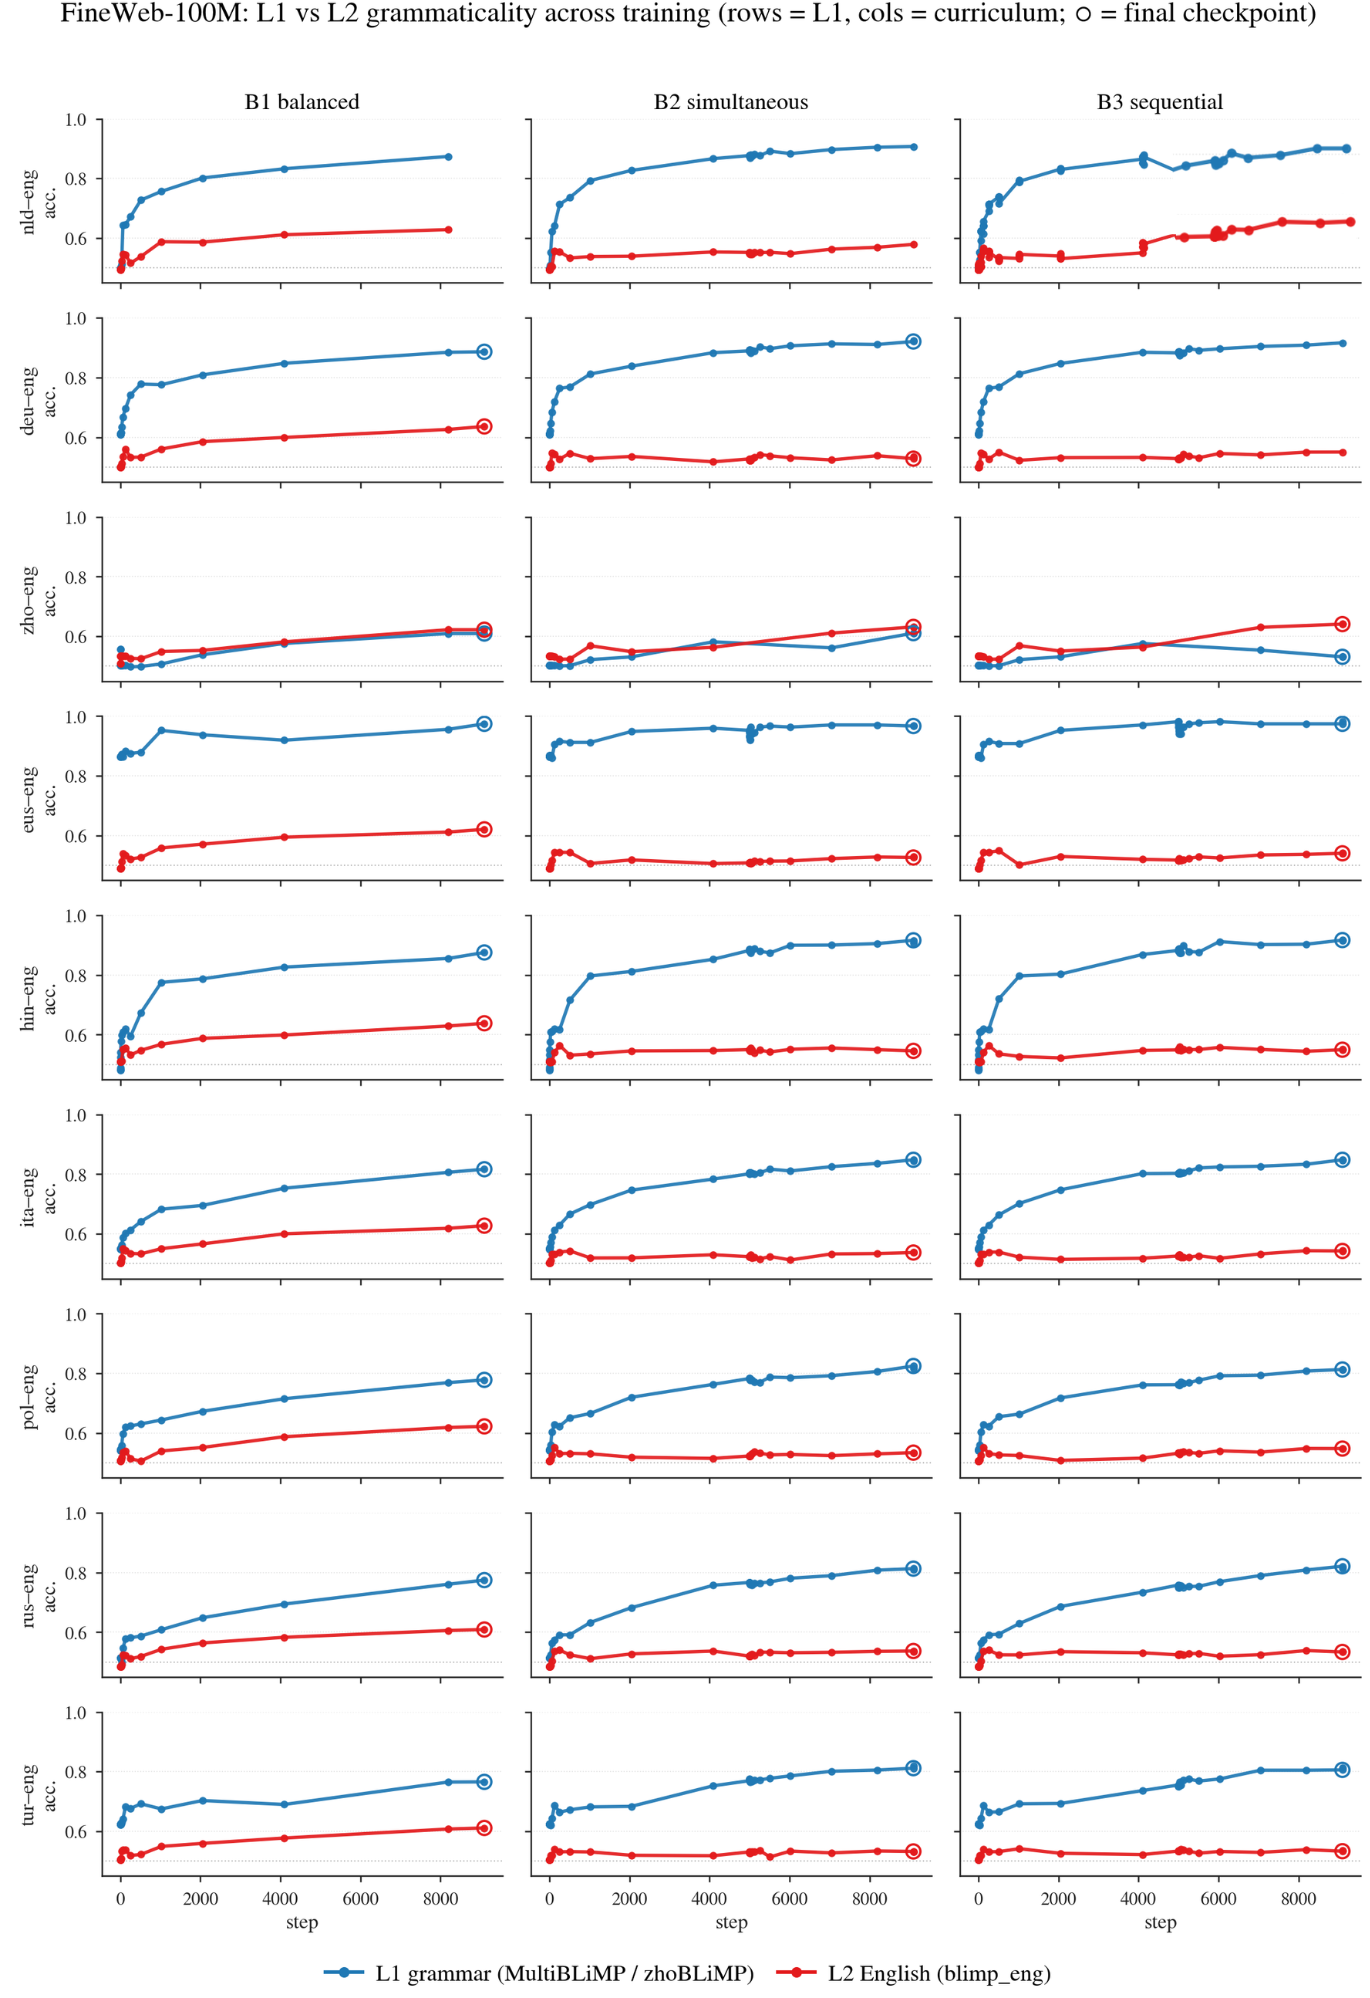
\includegraphics[width=\linewidth]{fig/b1-b3-blimps-checkpoints.png}
    \caption{Caption}
    \label{fig:blimp-checkpoints-beetle}
\end{figure*}
\clearpage 
\newpage 
\section{Detailed \beetle{} BLiSS Results}

\subsubsection{\beetle{} BLiSS Performance}

% Two-column layout of the Beetle BLiSS results, grouped by L1.
% Requires: \usepackage{booktabs,array}; \usepackage[table]{xcolor}
% Drops seed runs, ablations (episodic/alibi/ewc/lamol/pre-pretrain),
% the B3 (0--100) variant, FW-24B runs, and pending (\pend) rows.
% Bold = per-L1 column maximum.
\begin{table*}[t]
\centering\scriptsize
\setlength{\tabcolsep}{3pt}
\begin{minipage}[t]{0.49\linewidth}\centering
\begin{tabular}{ll l cccc}
\toprule
& & & \multicolumn{4}{c}{\textbf{BLiSS (matched-L1 cohort)}} \\
\cmidrule(lr){4-7}
\textbf{Pair} & \textbf{Data} & \textbf{Curr.} & \textbf{RP@0} & \textbf{RP@$\tau$} & \textbf{NGS} & \textbf{CPS} \\
\midrule
\texttt{deu--eng} & Human-scale & Mono & \cellcolor[rgb]{0.990,1.000,0.990} 51.0 & \cellcolor[rgb]{1.000,0.887,0.887} 38.3 & \cellcolor[rgb]{0.983,1.000,0.983} 51.3 & \cellcolor[rgb]{1.000,0.774,0.774} 29.5 \\
 & Human-scale & B1 balanced & \cellcolor[rgb]{0.925,1.000,0.925} \textbf{57.2} & \cellcolor[rgb]{1.000,0.983,0.983} \textbf{48.2} & \cellcolor[rgb]{0.927,1.000,0.927} 55.5 & \cellcolor[rgb]{1.000,0.965,0.965} 46.8 \\
 & Human-scale & B2 simult. & \cellcolor[rgb]{0.950,1.000,0.950} 54.8 & \cellcolor[rgb]{1.000,0.947,0.947} 44.5 & \cellcolor[rgb]{0.935,1.000,0.935} 54.9 & \cellcolor[rgb]{1.000,0.836,0.836} 35.1 \\
 & Human-scale & B3 sequential & \cellcolor[rgb]{0.943,1.000,0.943} 55.5 & \cellcolor[rgb]{1.000,0.971,0.971} 47.0 & \cellcolor[rgb]{0.927,1.000,0.927} 55.5 & \cellcolor[rgb]{1.000,0.853,0.853} 36.7 \\
 & Human-scale & B4 classroom & \cellcolor[rgb]{0.950,1.000,0.950} 54.8 & \cellcolor[rgb]{1.000,0.942,0.942} 44.0 & \cellcolor[rgb]{0.938,1.000,0.938} 54.7 & \cellcolor[rgb]{1.000,0.882,0.882} 39.3 \\
 & Human-scale & B5 late & \cellcolor[rgb]{0.946,1.000,0.946} 55.2 & \cellcolor[rgb]{1.000,0.951,0.951} 44.9 & \cellcolor[rgb]{0.939,1.000,0.939} 54.6 & \cellcolor[rgb]{1.000,0.839,0.839} 35.4 \\
\addlinespace[1.5pt]
 & 100M tok & B1 balanced & \cellcolor[rgb]{0.952,1.000,0.952} 54.6 & \cellcolor[rgb]{1.000,0.960,0.960} 45.8 & \cellcolor[rgb]{0.942,1.000,0.942} 54.4 & \cellcolor[rgb]{0.998,1.000,0.998} 50.1 \\
 & 100M tok & B2 simult. & \cellcolor[rgb]{0.942,1.000,0.942} 55.6 & \cellcolor[rgb]{1.000,0.972,0.972} 47.1 & \cellcolor[rgb]{0.918,1.000,0.918} \textbf{56.2} & \cellcolor[rgb]{1.000,0.891,0.891} 40.1 \\
 & 100M tok & B3 sequential & \cellcolor[rgb]{0.942,1.000,0.942} 55.6 & \cellcolor[rgb]{1.000,0.955,0.955} 45.3 & \cellcolor[rgb]{0.934,1.000,0.934} 55.0 & \cellcolor[rgb]{1.000,0.870,0.870} 38.2 \\
 & 100M tok & B4 classroom & \cellcolor[rgb]{0.949,1.000,0.949} 54.9 & \cellcolor[rgb]{1.000,0.957,0.957} 45.5 & \cellcolor[rgb]{0.925,1.000,0.925} 55.7 & \cellcolor[rgb]{1.000,0.934,0.934} 44.0 \\
 & 100M tok & B5 late & \cellcolor[rgb]{0.936,1.000,0.936} 56.1 & \cellcolor[rgb]{1.000,0.972,0.972} 47.1 & \cellcolor[rgb]{0.930,1.000,0.930} 55.3 & \cellcolor[rgb]{1.000,0.979,0.979} 48.1 \\
\addlinespace[1.5pt]
 & 2B tok & B1 balanced & \cellcolor[rgb]{0.964,1.000,0.964} 53.5 & \cellcolor[rgb]{1.000,0.937,0.937} 43.5 & \cellcolor[rgb]{0.955,1.000,0.955} 53.4 & \cellcolor[rgb]{1.000,0.986,0.986} 48.7 \\
 & 2B tok & B2 simult. & \cellcolor[rgb]{0.943,1.000,0.943} 55.5 & \cellcolor[rgb]{1.000,0.962,0.962} 46.1 & \cellcolor[rgb]{0.934,1.000,0.934} 55.0 & \cellcolor[rgb]{1.000,0.967,0.967} 47.0 \\
 & 2B tok & B3 sequential & \cellcolor[rgb]{0.964,1.000,0.964} 53.5 & \cellcolor[rgb]{1.000,0.960,0.960} 45.8 & \cellcolor[rgb]{0.951,1.000,0.951} 53.7 & \cellcolor[rgb]{1.000,0.999,0.999} 49.9 \\
 & 2B tok & B4 classroom & \cellcolor[rgb]{0.941,1.000,0.941} 55.7 & \cellcolor[rgb]{1.000,0.954,0.954} 45.2 & \cellcolor[rgb]{0.926,1.000,0.926} 55.6 & \cellcolor[rgb]{1.000,0.934,0.934} 44.0 \\
 & 2B tok & B5 late & \cellcolor[rgb]{0.937,1.000,0.937} 56.0 & \cellcolor[rgb]{1.000,0.949,0.949} 44.7 & \cellcolor[rgb]{0.931,1.000,0.931} 55.2 & \cellcolor[rgb]{1.000,0.978,0.978} 48.0 \\
\addlinespace[1.5pt]
 & 24B tok & B1 balanced & \cellcolor[rgb]{0.968,1.000,0.968} 53.1 & \cellcolor[rgb]{1.000,0.969,0.969} 46.8 & \cellcolor[rgb]{0.960,1.000,0.960} 53.0 & \cellcolor[rgb]{0.959,1.000,0.959} \textbf{52.0} \\
 & 24B tok & B2 simult. & \cellcolor[rgb]{0.949,1.000,0.949} 54.9 & \cellcolor[rgb]{1.000,0.964,0.964} 46.3 & \cellcolor[rgb]{0.926,1.000,0.926} 55.6 & \cellcolor[rgb]{1.000,0.957,0.957} 46.1 \\
\midrule
\texttt{nld--eng} & Human-scale & Mono & \cellcolor[rgb]{0.945,1.000,0.945} 55.3 & \cellcolor[rgb]{1.000,0.948,0.948} 44.6 & \cellcolor[rgb]{0.939,1.000,0.939} 54.6 & \cellcolor[rgb]{1.000,0.805,0.805} 32.3 \\
 & Human-scale & B1 balanced & \cellcolor[rgb]{0.931,1.000,0.931} 56.6 & \cellcolor[rgb]{1.000,0.989,0.989} 48.9 & \cellcolor[rgb]{0.931,1.000,0.931} 55.2 & \cellcolor[rgb]{1.000,0.982,0.982} 48.4 \\
 & Human-scale & B2 simult. & \cellcolor[rgb]{0.922,1.000,0.922} 57.5 & \cellcolor[rgb]{0.999,1.000,0.999} 50.1 & \cellcolor[rgb]{0.902,1.000,0.902} 57.4 & \cellcolor[rgb]{1.000,0.874,0.874} 38.6 \\
 & Human-scale & B3 sequential & \cellcolor[rgb]{0.920,1.000,0.920} 57.7 & \cellcolor[rgb]{1.000,0.991,0.991} 49.1 & \cellcolor[rgb]{0.907,1.000,0.907} 57.0 & \cellcolor[rgb]{1.000,0.893,0.893} 40.3 \\
 & Human-scale & B4 classroom & \cellcolor[rgb]{0.924,1.000,0.924} 57.3 & \cellcolor[rgb]{1.000,0.977,0.977} 47.6 & \cellcolor[rgb]{0.923,1.000,0.923} 55.8 & \cellcolor[rgb]{1.000,0.915,0.915} 42.3 \\
 & Human-scale & B5 late & \cellcolor[rgb]{0.926,1.000,0.926} 57.1 & \cellcolor[rgb]{1.000,0.987,0.987} 48.6 & \cellcolor[rgb]{0.911,1.000,0.911} 56.7 & \cellcolor[rgb]{1.000,0.881,0.881} 39.2 \\
\addlinespace[1.5pt]
 & 100M tok & B1 balanced & \cellcolor[rgb]{0.926,1.000,0.926} 57.1 & \cellcolor[rgb]{0.999,1.000,0.999} 50.1 & \cellcolor[rgb]{0.905,1.000,0.905} 57.2 & \cellcolor[rgb]{1.000,0.988,0.988} 48.9 \\
 & 100M tok & B2 simult. & \cellcolor[rgb]{0.901,1.000,0.901} 59.5 & \cellcolor[rgb]{0.997,1.000,0.997} 50.2 & \cellcolor[rgb]{0.890,1.000,0.890} \textbf{58.3} & \cellcolor[rgb]{1.000,0.898,0.898} 40.7 \\
 & 100M tok & B3 sequential & \cellcolor[rgb]{0.903,1.000,0.903} 59.3 & \cellcolor[rgb]{0.995,1.000,0.995} 50.4 & \cellcolor[rgb]{0.903,1.000,0.903} 57.3 & \cellcolor[rgb]{1.000,0.893,0.893} 40.3 \\
 & 100M tok & B4 classroom & \cellcolor[rgb]{0.918,1.000,0.918} 57.9 & \cellcolor[rgb]{1.000,0.998,0.998} 49.8 & \cellcolor[rgb]{0.905,1.000,0.905} 57.2 & \cellcolor[rgb]{1.000,0.906,0.906} 41.5 \\
 & 100M tok & B5 late & \cellcolor[rgb]{0.926,1.000,0.926} 57.1 & \cellcolor[rgb]{1.000,0.990,0.990} 49.0 & \cellcolor[rgb]{0.909,1.000,0.909} 56.9 & \cellcolor[rgb]{1.000,0.987,0.987} 48.8 \\
\addlinespace[1.5pt]
 & 2B tok & B1 balanced & \cellcolor[rgb]{0.911,1.000,0.911} 58.5 & \cellcolor[rgb]{0.992,1.000,0.992} 50.6 & \cellcolor[rgb]{0.907,1.000,0.907} 57.0 & \cellcolor[rgb]{1.000,0.975,0.975} 47.7 \\
 & 2B tok & B2 simult. & \cellcolor[rgb]{0.923,1.000,0.923} 57.4 & \cellcolor[rgb]{0.997,1.000,0.997} 50.2 & \cellcolor[rgb]{0.898,1.000,0.898} 57.7 & \cellcolor[rgb]{1.000,0.885,0.885} 39.6 \\
 & 2B tok & B3 sequential & \cellcolor[rgb]{0.916,1.000,0.916} 58.1 & \cellcolor[rgb]{1.000,0.991,0.991} 49.1 & \cellcolor[rgb]{0.897,1.000,0.897} 57.8 & \cellcolor[rgb]{1.000,0.860,0.860} 37.3 \\
 & 2B tok & B4 classroom & \cellcolor[rgb]{0.907,1.000,0.907} 58.9 & \cellcolor[rgb]{1.000,0.999,0.999} 49.9 & \cellcolor[rgb]{0.898,1.000,0.898} 57.7 & \cellcolor[rgb]{1.000,0.881,0.881} 39.2 \\
 & 2B tok & B5 late & \cellcolor[rgb]{0.909,1.000,0.909} 58.7 & \cellcolor[rgb]{0.995,1.000,0.995} 50.4 & \cellcolor[rgb]{0.899,1.000,0.899} 57.6 & \cellcolor[rgb]{1.000,0.851,0.851} 36.5 \\
\addlinespace[1.5pt]
 & 24B tok & B1 balanced & \cellcolor[rgb]{0.931,1.000,0.931} 56.6 & \cellcolor[rgb]{1.000,0.987,0.987} 48.6 & \cellcolor[rgb]{0.935,1.000,0.935} 54.9 & \cellcolor[rgb]{0.861,1.000,0.861} \textbf{56.8} \\
 & 24B tok & B2 simult. & \cellcolor[rgb]{0.896,1.000,0.896} 60.0 & \cellcolor[rgb]{0.976,1.000,0.976} 51.9 & \cellcolor[rgb]{0.895,1.000,0.895} 57.9 & \cellcolor[rgb]{0.969,1.000,0.969} 51.5 \\
 & 24B tok & B3 sequential & \cellcolor[rgb]{0.874,1.000,0.874} \textbf{62.1} & \cellcolor[rgb]{0.972,1.000,0.972} \textbf{52.2} & \cellcolor[rgb]{0.893,1.000,0.893} 58.1 & \cellcolor[rgb]{0.998,1.000,0.998} 50.1 \\
\bottomrule
\end{tabular}
\end{minipage}\hfill
\begin{minipage}[t]{0.49\linewidth}\centering
\begin{tabular}{ll l cccc}
\toprule
& & & \multicolumn{4}{c}{\textbf{BLiSS (matched-L1 cohort)}} \\
\cmidrule(lr){4-7}
\textbf{Pair} & \textbf{Data} & \textbf{Curr.} & \textbf{RP@0} & \textbf{RP@$\tau$} & \textbf{NGS} & \textbf{CPS} \\
\midrule
\texttt{zho--eng} & Human-scale & Mono & \cellcolor[rgb]{1.000,0.730,0.730} 45.4 & \cellcolor[rgb]{1.000,0.730,0.730} 22.0 & \cellcolor[rgb]{1.000,0.730,0.730} 46.5 & \cellcolor[rgb]{1.000,0.730,0.730} 25.5 \\
 & Human-scale & B2 simult. & \cellcolor[rgb]{0.856,1.000,0.856} 63.8 & \cellcolor[rgb]{0.942,1.000,0.942} 54.6 & \cellcolor[rgb]{0.857,1.000,0.857} 60.8 & \cellcolor[rgb]{1.000,0.851,0.851} 36.5 \\
 & Human-scale & B3 sequential & \cellcolor[rgb]{0.854,1.000,0.854} 64.0 & \cellcolor[rgb]{0.958,1.000,0.958} 53.3 & \cellcolor[rgb]{0.848,1.000,0.848} 61.5 & \cellcolor[rgb]{1.000,0.850,0.850} 36.4 \\
 & Human-scale & B5 late & \cellcolor[rgb]{0.851,1.000,0.851} 64.3 & \cellcolor[rgb]{0.937,1.000,0.937} 55.0 & \cellcolor[rgb]{0.843,1.000,0.843} 61.9 & \cellcolor[rgb]{1.000,0.850,0.850} 36.4 \\
\addlinespace[1.5pt]
 & 2B tok & B1 balanced & \cellcolor[rgb]{0.807,1.000,0.807} 68.5 & \cellcolor[rgb]{0.873,1.000,0.873} 60.1 & \cellcolor[rgb]{0.807,1.000,0.807} 64.6 & \cellcolor[rgb]{1.000,0.994,0.994} 49.5 \\
 & 2B tok & B2 simult. & \cellcolor[rgb]{0.808,1.000,0.808} 68.4 & \cellcolor[rgb]{0.886,1.000,0.886} 59.0 & \cellcolor[rgb]{0.813,1.000,0.813} 64.1 & \cellcolor[rgb]{1.000,0.983,0.983} 48.5 \\
 & 2B tok & B3 sequential & \cellcolor[rgb]{0.801,1.000,0.801} 69.1 & \cellcolor[rgb]{0.871,1.000,0.871} 60.2 & \cellcolor[rgb]{0.805,1.000,0.805} 64.7 & \cellcolor[rgb]{1.000,0.989,0.989} 49.0 \\
 & 2B tok & B4 classroom & \cellcolor[rgb]{0.846,1.000,0.846} 64.8 & \cellcolor[rgb]{0.923,1.000,0.923} 56.1 & \cellcolor[rgb]{0.823,1.000,0.823} 63.4 & \cellcolor[rgb]{1.000,0.905,0.905} 41.4 \\
 & 2B tok & B5 late & \cellcolor[rgb]{0.817,1.000,0.817} 67.6 & \cellcolor[rgb]{0.900,1.000,0.900} 57.9 & \cellcolor[rgb]{0.808,1.000,0.808} 64.5 & \cellcolor[rgb]{1.000,0.949,0.949} 45.4 \\
 \addlinespace[1.5pt]
 & 24B tok (FW-24B) & B1 balanced & \cellcolor[rgb]{0.796,1.000,0.796} 69.8 & \cellcolor[rgb]{0.856,1.000,0.856} 61.7 & \cellcolor[rgb]{0.804,1.000,0.804} 64.8 & \cellcolor[rgb]{1.000,0.932,0.932} 54.8 \\
 & 24B tok (FW-24B) & B2 simult. & \cellcolor[rgb]{0.792,1.000,0.792} 70.2 & \cellcolor[rgb]{0.849,1.000,0.849} 62.4 & \cellcolor[rgb]{0.804,1.000,0.804} 64.8 & \cellcolor[rgb]{1.000,0.934,0.934} 54.6 \\
 & 24B tok (FW-24B) & B3 sequential & \cellcolor[rgb]{0.811,1.000,0.811} 68.3 & \cellcolor[rgb]{0.859,1.000,0.859} 61.2 & \cellcolor[rgb]{0.816,1.000,0.816} 63.6 & \cellcolor[rgb]{1.000,0.928,0.928} 55.2 \\
 & 24B tok (FW-24B) & B3 sequential {\scriptsize\textit{ewc}} & \cellcolor[rgb]{0.796,1.000,0.796} 69.8 & \cellcolor[rgb]{0.858,1.000,0.858} 61.3 & \cellcolor[rgb]{0.810,1.000,0.810} 64.2 & \cellcolor[rgb]{1.000,0.919,0.919} \textbf{56.1} \\
 & 24B tok (FW-24B) & B4 classroom & \cellcolor[rgb]{0.804,1.000,0.804} 69.0 & \cellcolor[rgb]{0.852,1.000,0.852} 62.1 & \cellcolor[rgb]{0.805,1.000,0.805} 64.7 & \cellcolor[rgb]{1.000,0.961,0.961} 51.9 \\
 & 24B tok (FW-24B) & B5 late & \cellcolor[rgb]{0.787,1.000,0.787} \textbf{70.7} & \cellcolor[rgb]{0.843,1.000,0.843} \textbf{63.3} & \cellcolor[rgb]{0.802,1.000,0.802} \textbf{65.0} & \cellcolor[rgb]{1.000,0.942,0.942} 53.8 \\
\midrule
\midrule
\texttt{hin--eng} & 100M tok & B1 balanced & \cellcolor[rgb]{0.950,1.000,0.950} \textbf{54.8} & \cellcolor[rgb]{1.000,0.945,0.945} \textbf{44.3} & \cellcolor[rgb]{0.943,1.000,0.943} \textbf{54.3} & \cellcolor[rgb]{0.922,1.000,0.922} \textbf{53.8} \\
 & 100M tok & B2 simult. & \cellcolor[rgb]{0.975,1.000,0.975} 52.4 & \cellcolor[rgb]{1.000,0.910,0.910} 40.7 & \cellcolor[rgb]{0.952,1.000,0.952} 53.6 & \cellcolor[rgb]{1.000,0.917,0.917} 42.5 \\
 & 100M tok & B3 sequential & \cellcolor[rgb]{0.978,1.000,0.978} 52.1 & \cellcolor[rgb]{1.000,0.913,0.913} 41.0 & \cellcolor[rgb]{0.952,1.000,0.952} 53.6 & \cellcolor[rgb]{1.000,0.936,0.936} 44.2 \\
 & 100M tok & B4 classroom & \cellcolor[rgb]{0.955,1.000,0.955} 54.3 & \cellcolor[rgb]{1.000,0.918,0.918} 41.5 & \cellcolor[rgb]{0.948,1.000,0.948} 53.9 & \cellcolor[rgb]{1.000,0.964,0.964} 46.7 \\
 & 100M tok & B5 late & \cellcolor[rgb]{0.953,1.000,0.953} 54.5 & \cellcolor[rgb]{1.000,0.939,0.939} 43.7 & \cellcolor[rgb]{0.951,1.000,0.951} 53.7 & \cellcolor[rgb]{0.939,1.000,0.939} 53.0 \\
\addlinespace[1.5pt]
 & 2B tok & B2 simult. & \cellcolor[rgb]{0.969,1.000,0.969} 53.0 & \cellcolor[rgb]{1.000,0.910,0.910} 40.7 & \cellcolor[rgb]{0.960,1.000,0.960} 53.0 & \cellcolor[rgb]{1.000,0.910,0.910} 41.8 \\
\midrule
\texttt{ita--eng} & 100M tok & B1 balanced & \cellcolor[rgb]{0.869,1.000,0.869} \textbf{62.6} & \cellcolor[rgb]{0.984,1.000,0.984} \textbf{51.3} & \cellcolor[rgb]{0.872,1.000,0.872} 59.7 & \cellcolor[rgb]{1.000,0.992,0.992} \textbf{49.3} \\
 & 100M tok & B2 simult. & \cellcolor[rgb]{0.877,1.000,0.877} 61.8 & \cellcolor[rgb]{1.000,0.994,0.994} 49.4 & \cellcolor[rgb]{0.857,1.000,0.857} \textbf{60.8} & \cellcolor[rgb]{1.000,0.869,0.869} 38.1 \\
 & 100M tok & B3 sequential & \cellcolor[rgb]{0.874,1.000,0.874} 62.1 & \cellcolor[rgb]{1.000,0.986,0.986} 48.5 & \cellcolor[rgb]{0.870,1.000,0.870} 59.8 & \cellcolor[rgb]{1.000,0.871,0.871} 38.3 \\
 & 100M tok & B4 classroom & \cellcolor[rgb]{0.869,1.000,0.869} \textbf{62.6} & \cellcolor[rgb]{0.996,1.000,0.996} 50.3 & \cellcolor[rgb]{0.858,1.000,0.858} 60.7 & \cellcolor[rgb]{1.000,0.928,0.928} 43.5 \\
 & 100M tok & B5 late & \cellcolor[rgb]{0.880,1.000,0.880} 61.5 & \cellcolor[rgb]{0.992,1.000,0.992} 50.6 & \cellcolor[rgb]{0.873,1.000,0.873} 59.6 & \cellcolor[rgb]{1.000,0.972,0.972} 47.5 \\
\addlinespace[1.5pt]
 & 2B tok & B3 sequential & \cellcolor[rgb]{0.883,1.000,0.883} 61.2 & \cellcolor[rgb]{0.996,1.000,0.996} 50.3 & \cellcolor[rgb]{0.884,1.000,0.884} 58.8 & \cellcolor[rgb]{1.000,0.979,0.979} 48.1 \\
\midrule
\texttt{pol--eng} & 100M tok & B1 balanced & \cellcolor[rgb]{0.948,1.000,0.948} \textbf{55.0} & \cellcolor[rgb]{1.000,0.972,0.972} \textbf{47.1} & \cellcolor[rgb]{0.943,1.000,0.943} \textbf{54.3} & \cellcolor[rgb]{0.906,1.000,0.906} \textbf{54.6} \\
 & 100M tok & B2 simult. & \cellcolor[rgb]{0.977,1.000,0.977} 52.2 & \cellcolor[rgb]{1.000,0.941,0.941} 43.9 & \cellcolor[rgb]{0.959,1.000,0.959} 53.1 & \cellcolor[rgb]{1.000,0.946,0.946} 45.1 \\
 & 100M tok & B3 sequential & \cellcolor[rgb]{0.978,1.000,0.978} 52.1 & \cellcolor[rgb]{1.000,0.941,0.941} 43.9 & \cellcolor[rgb]{0.963,1.000,0.963} 52.8 & \cellcolor[rgb]{1.000,0.960,0.960} 46.4 \\
\midrule
\texttt{tur--eng} & 100M tok & B1 balanced & \cellcolor[rgb]{0.922,1.000,0.922} \textbf{57.5} & \cellcolor[rgb]{0.997,1.000,0.997} \textbf{50.2} & \cellcolor[rgb]{0.925,1.000,0.925} \textbf{55.7} & \cellcolor[rgb]{0.988,1.000,0.988} \textbf{50.6} \\
 & 100M tok & B2 simult. & \cellcolor[rgb]{0.967,1.000,0.967} 53.2 & \cellcolor[rgb]{1.000,0.951,0.951} 44.9 & \cellcolor[rgb]{0.956,1.000,0.956} 53.3 & \cellcolor[rgb]{1.000,0.888,0.888} 39.8 \\
 & 100M tok & B3 sequential & \cellcolor[rgb]{0.971,1.000,0.971} 52.8 & \cellcolor[rgb]{1.000,0.950,0.950} 44.8 & \cellcolor[rgb]{0.958,1.000,0.958} 53.2 & \cellcolor[rgb]{1.000,0.881,0.881} 39.2 \\
 & 100M tok & B4 classroom & \cellcolor[rgb]{0.934,1.000,0.934} 56.3 & \cellcolor[rgb]{1.000,0.984,0.984} 48.3 & \cellcolor[rgb]{0.926,1.000,0.926} 55.6 & \cellcolor[rgb]{1.000,0.923,0.923} 43.0 \\
 & 100M tok & B5 late & \cellcolor[rgb]{0.936,1.000,0.936} 56.1 & \cellcolor[rgb]{1.000,0.991,0.991} 49.1 & \cellcolor[rgb]{0.929,1.000,0.929} 55.4 & \cellcolor[rgb]{1.000,0.986,0.986} 48.7 \\
\midrule
\texttt{eng--deu} & 24B tok & B1 balanced & \cellcolor[rgb]{0.952,1.000,0.952} \textbf{54.6} & \cellcolor[rgb]{1.000,0.964,0.964} \textbf{46.3} & \cellcolor[rgb]{0.962,1.000,0.962} \textbf{52.9} & \cellcolor[rgb]{0.963,1.000,0.963} \textbf{51.8} \\
\midrule
\texttt{eng--nld} & 24B tok & B1 balanced & \cellcolor[rgb]{0.929,1.000,0.929} \textbf{56.8} & \cellcolor[rgb]{0.997,1.000,0.997} \textbf{50.2} & \cellcolor[rgb]{0.938,1.000,0.938} \textbf{54.7} & \cellcolor[rgb]{0.904,1.000,0.904} 54.7 \\
 & 24B tok & B2 simult. & \cellcolor[rgb]{0.931,1.000,0.931} 56.6 & \cellcolor[rgb]{1.000,0.987,0.987} 48.6 & \cellcolor[rgb]{0.946,1.000,0.946} 54.1 & \cellcolor[rgb]{0.904,1.000,0.904} 54.7 \\
 & 24B tok & B3 sequential & \cellcolor[rgb]{0.952,1.000,0.952} 54.6 & \cellcolor[rgb]{1.000,0.979,0.979} 47.8 & \cellcolor[rgb]{0.955,1.000,0.955} 53.4 & \cellcolor[rgb]{0.881,1.000,0.881} \textbf{55.8} \\
\bottomrule
\end{tabular}
\end{minipage}
\caption{BLiSS learner-minimal-pair scores (\%, 0--100) for Beetle models on the \emph{matched-L1 cohort}, grouped by L1 then token budget. Cell shading encodes score on a fixed scale (darker green = higher). Per L1, the highest value in each metric column is shown in \textbf{bold}. Metrics: RP@0 / RP@$\tau$ (random-over-human preference, with and without a margin), NGS (normalised gap score), CPS (correct-preferred sanity check). Seed, method-ablation, FrameWork-2 runs and pending evaluations are reported separately in Table~\ref{tab:bliss_ablations}.}
\label{tab:bliss_beetle}
\end{table*}

\begin{table}[t]
\centering\small
\setlength{\tabcolsep}{4pt}
\begin{tabular}{ll l cc cc}
\toprule
& & & \multicolumn{2}{c}{\textbf{MultiBLiMP}} & \multicolumn{2}{c}{\textbf{MonoBLiMP}} \\
\cmidrule(lr){4-5}\cmidrule(lr){6-7}
\textbf{Model} & \textbf{Params} & \textbf{Cohort} & \textbf{L1} & \textbf{Eng} & \textbf{L1} & \textbf{Eng} \\
\midrule
\multirow{3}{*}{BLOOM-560M} & \multirow{3}{*}{0.56B} & Dutch & \cellcolor[rgb]{0.946,1.000,0.946} 59.8 & \cellcolor[rgb]{0.827,1.000,0.827} 81.7 & \cellcolor[rgb]{0.982,1.000,0.982} 52.6 & \cellcolor[rgb]{0.863,1.000,0.863} 66.7 \\
 &  & German & \cellcolor[rgb]{0.912,1.000,0.912} 65.9 & \cellcolor[rgb]{0.827,1.000,0.827} 81.7 & \na & \cellcolor[rgb]{0.863,1.000,0.863} 66.7 \\
 &  & Chinese & \na & \cellcolor[rgb]{0.827,1.000,0.827} 81.7 & \cellcolor[rgb]{0.840,1.000,0.840} 72.5 & \cellcolor[rgb]{0.863,1.000,0.863} 66.7 \\
\addlinespace[2pt]
\multirow{3}{*}{BLOOM-1.1B} & \multirow{3}{*}{1.1B} & Dutch & \cellcolor[rgb]{0.928,1.000,0.928} 63.0 & \cellcolor[rgb]{0.768,1.000,0.768} 92.5 & \cellcolor[rgb]{1.000,0.730,0.730} 48.7 & \cellcolor[rgb]{0.780,1.000,0.780} 76.7 \\
 &  & German & \cellcolor[rgb]{0.853,1.000,0.853} 76.5 & \cellcolor[rgb]{0.768,1.000,0.768} 92.5 & \na & \cellcolor[rgb]{0.780,1.000,0.780} 76.7 \\
 &  & Chinese & \na & \cellcolor[rgb]{0.768,1.000,0.768} 92.5 & \cellcolor[rgb]{0.758,1.000,0.758} 84.1 & \cellcolor[rgb]{0.780,1.000,0.780} 76.7 \\
\addlinespace[2pt]
\multirow{3}{*}{BLOOM-1.7B} & \multirow{3}{*}{1.7B} & Dutch & \cellcolor[rgb]{0.909,1.000,0.909} 66.4 & \cellcolor[rgb]{0.765,1.000,0.765} 93.0 & \cellcolor[rgb]{1.000,0.730,0.730} 48.7 & \cellcolor[rgb]{0.783,1.000,0.783} 76.4 \\
 &  & German & \cellcolor[rgb]{0.861,1.000,0.861} 75.2 & \cellcolor[rgb]{0.765,1.000,0.765} 93.0 & \na & \cellcolor[rgb]{0.783,1.000,0.783} 76.4 \\
 &  & Chinese & \na & \cellcolor[rgb]{0.765,1.000,0.765} 93.0 & \cellcolor[rgb]{0.753,1.000,0.753} 84.8 & \cellcolor[rgb]{0.783,1.000,0.783} 76.4 \\
\addlinespace[2pt]
\multirow{3}{*}{BLOOM-3B} & \multirow{3}{*}{3B} & Dutch & \cellcolor[rgb]{0.910,1.000,0.910} 66.3 & \cellcolor[rgb]{0.756,1.000,0.756} 94.8 & \cellcolor[rgb]{0.992,1.000,0.992} 51.1 & \cellcolor[rgb]{0.801,1.000,0.801} 74.2 \\
 &  & German & \cellcolor[rgb]{0.830,1.000,0.830} 80.7 & \cellcolor[rgb]{0.756,1.000,0.756} 94.8 & \na & \cellcolor[rgb]{0.801,1.000,0.801} 74.2 \\
 &  & Chinese & \na & \cellcolor[rgb]{0.756,1.000,0.756} 94.8 & \cellcolor[rgb]{0.758,1.000,0.758} 84.0 & \cellcolor[rgb]{0.801,1.000,0.801} 74.2 \\
\addlinespace[2pt]
\multirow{3}{*}{BLOOM-7.1B} & \multirow{3}{*}{7.1B} & Dutch & \cellcolor[rgb]{0.923,1.000,0.923} 64.0 & \cellcolor[rgb]{0.760,1.000,0.760} 94.0 & \cellcolor[rgb]{0.961,1.000,0.961} 55.5 & \cellcolor[rgb]{0.774,1.000,0.774} 77.5 \\
 &  & German & \cellcolor[rgb]{0.822,1.000,0.822} 82.2 & \cellcolor[rgb]{0.760,1.000,0.760} 94.0 & \na & \cellcolor[rgb]{0.774,1.000,0.774} 77.5 \\
 &  & Chinese & \na & \cellcolor[rgb]{0.760,1.000,0.760} 94.0 & \cellcolor[rgb]{0.756,1.000,0.756} 84.3 & \cellcolor[rgb]{0.774,1.000,0.774} 77.5 \\
\addlinespace[2pt]
\multirow{3}{*}{XGLM-4.5B} & \multirow{3}{*}{4.5B} & Dutch & \cellcolor[rgb]{0.741,1.000,0.741} 96.9 & \cellcolor[rgb]{0.734,1.000,0.734} 98.7 & \cellcolor[rgb]{0.761,1.000,0.761} 83.6 & \cellcolor[rgb]{0.746,1.000,0.746} 80.9 \\
 &  & German & \cellcolor[rgb]{0.730,1.000,0.730} 98.8 & \cellcolor[rgb]{0.734,1.000,0.734} 98.7 & \na & \cellcolor[rgb]{0.746,1.000,0.746} 80.9 \\
 &  & Chinese & \na & \cellcolor[rgb]{0.734,1.000,0.734} 98.7 & \cellcolor[rgb]{0.754,1.000,0.754} 84.6 & \cellcolor[rgb]{0.746,1.000,0.746} 80.9 \\
\addlinespace[2pt]
\multirow{3}{*}{EuroLLM-9B} & \multirow{3}{*}{9B} & Dutch & \cellcolor[rgb]{0.854,1.000,0.854} 76.4 & \cellcolor[rgb]{0.812,1.000,0.812} 84.4 & \cellcolor[rgb]{0.730,1.000,0.730} 88.0 & \cellcolor[rgb]{0.756,1.000,0.756} 79.6 \\
 &  & German & \cellcolor[rgb]{0.849,1.000,0.849} 77.3 & \cellcolor[rgb]{0.812,1.000,0.812} 84.4 & \na & \cellcolor[rgb]{0.756,1.000,0.756} 79.6 \\
 &  & Chinese & \na & \cellcolor[rgb]{0.812,1.000,0.812} 84.4 & \cellcolor[rgb]{0.762,1.000,0.762} 83.5 & \cellcolor[rgb]{0.756,1.000,0.756} 79.6 \\
\addlinespace[2pt]
\multirow{3}{*}{Gemma-3-270M} & \multirow{3}{*}{0.27B} & Dutch & \cellcolor[rgb]{0.814,1.000,0.814} 83.7 & \cellcolor[rgb]{0.744,1.000,0.744} 97.0 & \cellcolor[rgb]{0.859,1.000,0.859} 69.9 & \cellcolor[rgb]{0.763,1.000,0.763} 78.8 \\
 &  & German & \cellcolor[rgb]{0.776,1.000,0.776} 90.4 & \cellcolor[rgb]{0.744,1.000,0.744} 97.0 & \na & \cellcolor[rgb]{0.763,1.000,0.763} 78.8 \\
 &  & Chinese & \na & \cellcolor[rgb]{0.744,1.000,0.744} 97.0 & \cellcolor[rgb]{0.782,1.000,0.782} 80.7 & \cellcolor[rgb]{0.763,1.000,0.763} 78.8 \\
\addlinespace[2pt]
\multirow{3}{*}{Gemma-2-2B} & \multirow{3}{*}{2B} & Dutch & \cellcolor[rgb]{0.769,1.000,0.769} 91.7 & \cellcolor[rgb]{0.734,1.000,0.734} 98.7 & \cellcolor[rgb]{0.783,1.000,0.783} 80.5 & \cellcolor[rgb]{0.782,1.000,0.782} 76.5 \\
 &  & German & \cellcolor[rgb]{0.748,1.000,0.748} 95.6 & \cellcolor[rgb]{0.734,1.000,0.734} 98.7 & \na & \cellcolor[rgb]{0.782,1.000,0.782} 76.5 \\
 &  & Chinese & \na & \cellcolor[rgb]{0.734,1.000,0.734} 98.7 & \cellcolor[rgb]{0.770,1.000,0.770} 82.3 & \cellcolor[rgb]{0.782,1.000,0.782} 76.5 \\
\addlinespace[2pt]
\multirow{3}{*}{Gemma-2-9B} & \multirow{3}{*}{9B} & Dutch & \cellcolor[rgb]{0.772,1.000,0.772} 91.2 & \cellcolor[rgb]{0.734,1.000,0.734} 98.8 & \cellcolor[rgb]{0.756,1.000,0.756} 84.4 & \cellcolor[rgb]{0.775,1.000,0.775} 77.3 \\
 &  & German & \cellcolor[rgb]{0.743,1.000,0.743} 96.4 & \cellcolor[rgb]{0.734,1.000,0.734} 98.8 & \na & \cellcolor[rgb]{0.775,1.000,0.775} 77.3 \\
 &  & Chinese & \na & \cellcolor[rgb]{0.734,1.000,0.734} 98.8 & \cellcolor[rgb]{0.766,1.000,0.766} 82.9 & \cellcolor[rgb]{0.775,1.000,0.775} 77.3 \\
\addlinespace[2pt]
\multirow{3}{*}{Gemma-2-27B} & \multirow{3}{*}{27B} & Dutch & \cellcolor[rgb]{0.842,1.000,0.842} 78.6 & \cellcolor[rgb]{0.822,1.000,0.822} 82.6 & \cellcolor[rgb]{0.829,1.000,0.829} 74.0 & \cellcolor[rgb]{0.830,1.000,0.830} 70.7 \\
 &  & German & \cellcolor[rgb]{0.828,1.000,0.828} 81.1 & \cellcolor[rgb]{0.822,1.000,0.822} 82.6 & \na & \cellcolor[rgb]{0.830,1.000,0.830} 70.7 \\
 &  & Chinese & \na & \cellcolor[rgb]{0.822,1.000,0.822} 82.6 & \cellcolor[rgb]{0.847,1.000,0.847} 71.5 & \cellcolor[rgb]{0.830,1.000,0.830} 70.7 \\
\addlinespace[2pt]
\multirow{3}{*}{Qwen3-0.6B} & \multirow{3}{*}{0.6B} & Dutch & \cellcolor[rgb]{0.826,1.000,0.826} 81.5 & \cellcolor[rgb]{0.744,1.000,0.744} 97.0 & \cellcolor[rgb]{0.846,1.000,0.846} 71.7 & \cellcolor[rgb]{0.740,1.000,0.740} 81.6 \\
 &  & German & \cellcolor[rgb]{0.764,1.000,0.764} 92.6 & \cellcolor[rgb]{0.744,1.000,0.744} 97.0 & \na & \cellcolor[rgb]{0.740,1.000,0.740} 81.6 \\
 &  & Chinese & \na & \cellcolor[rgb]{0.744,1.000,0.744} 97.0 & \cellcolor[rgb]{0.773,1.000,0.773} 82.0 & \cellcolor[rgb]{0.740,1.000,0.740} 81.6 \\
\addlinespace[2pt]
\multirow{3}{*}{Qwen3-4B} & \multirow{3}{*}{4B} & Dutch & \cellcolor[rgb]{0.757,1.000,0.757} 93.9 & \cellcolor[rgb]{0.730,1.000,0.730} 99.5 & \cellcolor[rgb]{0.768,1.000,0.768} 82.6 & \cellcolor[rgb]{0.730,1.000,0.730} 82.8 \\
 &  & German & \cellcolor[rgb]{0.739,1.000,0.739} 97.2 & \cellcolor[rgb]{0.730,1.000,0.730} 99.5 & \na & \cellcolor[rgb]{0.730,1.000,0.730} 82.8 \\
 &  & Chinese & \na & \cellcolor[rgb]{0.730,1.000,0.730} 99.5 & \cellcolor[rgb]{0.745,1.000,0.745} 85.9 & \cellcolor[rgb]{0.730,1.000,0.730} 82.8 \\
\addlinespace[2pt]
\multirow{3}{*}{Qwen3-8B} & \multirow{3}{*}{8B} & Dutch & \cellcolor[rgb]{0.753,1.000,0.753} 94.6 & \cellcolor[rgb]{0.734,1.000,0.734} 98.7 & \cellcolor[rgb]{0.772,1.000,0.772} 82.1 & \cellcolor[rgb]{0.732,1.000,0.732} 82.5 \\
 &  & German & \cellcolor[rgb]{0.732,1.000,0.732} 98.5 & \cellcolor[rgb]{0.734,1.000,0.734} 98.7 & \na & \cellcolor[rgb]{0.732,1.000,0.732} 82.5 \\
 &  & Chinese & \na & \cellcolor[rgb]{0.734,1.000,0.734} 98.7 & \cellcolor[rgb]{0.745,1.000,0.745} 85.9 & \cellcolor[rgb]{0.732,1.000,0.732} 82.5 \\
\addlinespace[2pt]
\multirow{3}{*}{Llama-3.2-1B} & \multirow{3}{*}{1B} & Dutch & \cellcolor[rgb]{0.774,1.000,0.774} 90.8 & \cellcolor[rgb]{0.733,1.000,0.733} 99.0 & \cellcolor[rgb]{0.815,1.000,0.815} 76.0 & \cellcolor[rgb]{0.738,1.000,0.738} 81.8 \\
 &  & German & \cellcolor[rgb]{0.745,1.000,0.745} 96.1 & \cellcolor[rgb]{0.733,1.000,0.733} 99.0 & \na & \cellcolor[rgb]{0.738,1.000,0.738} 81.8 \\
 &  & Chinese & \na & \cellcolor[rgb]{0.733,1.000,0.733} 99.0 & \cellcolor[rgb]{0.766,1.000,0.766} 82.9 & \cellcolor[rgb]{0.738,1.000,0.738} 81.8 \\
\addlinespace[2pt]
\multirow{3}{*}{Llama-3.1-8B} & \multirow{3}{*}{8B} & Dutch & \cellcolor[rgb]{0.745,1.000,0.745} 96.1 & \cellcolor[rgb]{0.732,1.000,0.732} 99.2 & \cellcolor[rgb]{0.751,1.000,0.751} 85.1 & \cellcolor[rgb]{0.743,1.000,0.743} 81.2 \\
 &  & German & \cellcolor[rgb]{0.734,1.000,0.734} 98.0 & \cellcolor[rgb]{0.732,1.000,0.732} 99.2 & \na & \cellcolor[rgb]{0.743,1.000,0.743} 81.2 \\
 &  & Chinese & \na & \cellcolor[rgb]{0.732,1.000,0.732} 99.2 & \cellcolor[rgb]{0.755,1.000,0.755} 84.5 & \cellcolor[rgb]{0.743,1.000,0.743} 81.2 \\
\bottomrule
\end{tabular}
\caption{Frontier multilingual-LLM baselines \emph{Params} is the parameter count; \emph{Cohort} is the evaluation language.}
\label{tab:baselines}
\end{table}





\clearpage
\newpage 
\subsubsection{BLiSS LLM Baselines}
% Two-column layout of the BLiSS frontier-LLM baselines.
% Requires: \usepackage{booktabs,array}; \usepackage[table]{xcolor}
% Bold = per-model column maximum across its three L1 cohort rows.
\begin{table*}[t]
\centering\scriptsize
\setlength{\tabcolsep}{3pt}
\begin{minipage}[t]{0.49\linewidth}\centering
\begin{tabular}{ll l cccc}
\toprule
& & & \multicolumn{4}{c}{\textbf{BLiSS (matched-L1 cohort)}} \\
\cmidrule(lr){4-7}
\textbf{Model} & \textbf{Params} & \textbf{L1} & \textbf{RP@0} & \textbf{RP@$\tau$} & \textbf{NGS} & \textbf{CPS} \\
\midrule
BLOOM-560M & 0.56B & Dutch & \cellcolor[rgb]{0.906,1.000,0.906} 59.0 & \cellcolor[rgb]{0.966,1.000,0.966} 52.7 & \cellcolor[rgb]{0.929,1.000,0.929} 55.4 & \cellcolor[rgb]{0.881,1.000,0.881} 55.8 \\
 &  & German & \cellcolor[rgb]{0.907,1.000,0.907} 58.9 & \cellcolor[rgb]{0.991,1.000,0.991} 50.7 & \cellcolor[rgb]{0.935,1.000,0.935} 54.9 & \cellcolor[rgb]{0.953,1.000,0.953} 52.3 \\
 &  & Chinese & \cellcolor[rgb]{0.789,1.000,0.789} \textbf{70.2} & \cellcolor[rgb]{0.847,1.000,0.847} \textbf{62.1} & \cellcolor[rgb]{0.801,1.000,0.801} \textbf{65.0} & \cellcolor[rgb]{0.875,1.000,0.875} \textbf{56.1} \\
\addlinespace[2pt]
BLOOM-1.1B & 1.1B & Dutch & \cellcolor[rgb]{0.899,1.000,0.899} 59.7 & \cellcolor[rgb]{0.980,1.000,0.980} 51.6 & \cellcolor[rgb]{0.923,1.000,0.923} 55.8 & \cellcolor[rgb]{0.865,1.000,0.865} \textbf{56.6} \\
 &  & German & \cellcolor[rgb]{0.921,1.000,0.921} 57.6 & \cellcolor[rgb]{1.000,0.994,0.994} 49.4 & \cellcolor[rgb]{0.938,1.000,0.938} 54.7 & \cellcolor[rgb]{0.937,1.000,0.937} 53.1 \\
 &  & Chinese & \cellcolor[rgb]{0.788,1.000,0.788} \textbf{70.3} & \cellcolor[rgb]{0.828,1.000,0.828} \textbf{63.6} & \cellcolor[rgb]{0.792,1.000,0.792} \textbf{65.7} & \cellcolor[rgb]{0.865,1.000,0.865} \textbf{56.6} \\
\addlinespace[2pt]
BLOOM-1.7B & 1.7B & Dutch & \cellcolor[rgb]{0.906,1.000,0.906} 59.0 & \cellcolor[rgb]{0.984,1.000,0.984} 51.3 & \cellcolor[rgb]{0.922,1.000,0.922} 55.9 & \cellcolor[rgb]{0.865,1.000,0.865} 56.6 \\
 &  & German & \cellcolor[rgb]{0.924,1.000,0.924} 57.3 & \cellcolor[rgb]{0.997,1.000,0.997} 50.2 & \cellcolor[rgb]{0.938,1.000,0.938} 54.7 & \cellcolor[rgb]{0.883,1.000,0.883} 55.7 \\
 &  & Chinese & \cellcolor[rgb]{0.786,1.000,0.786} \textbf{70.5} & \cellcolor[rgb]{0.827,1.000,0.827} \textbf{63.7} & \cellcolor[rgb]{0.792,1.000,0.792} \textbf{65.7} & \cellcolor[rgb]{0.828,1.000,0.828} \textbf{58.4} \\
\addlinespace[2pt]
BLOOM-7.1B & 7.1B & Dutch & \cellcolor[rgb]{0.863,1.000,0.863} 63.1 & \cellcolor[rgb]{0.909,1.000,0.909} 57.2 & \cellcolor[rgb]{0.890,1.000,0.890} 58.3 & \cellcolor[rgb]{0.820,1.000,0.820} \textbf{58.8} \\
 &  & German & \cellcolor[rgb]{0.903,1.000,0.903} 59.3 & \cellcolor[rgb]{0.999,1.000,0.999} 50.0 & \cellcolor[rgb]{0.925,1.000,0.925} 55.7 & \cellcolor[rgb]{0.863,1.000,0.863} 56.7 \\
 &  & Chinese & \cellcolor[rgb]{0.758,1.000,0.758} \textbf{73.2} & \cellcolor[rgb]{0.803,1.000,0.803} \textbf{65.6} & \cellcolor[rgb]{0.770,1.000,0.770} \textbf{67.4} & \cellcolor[rgb]{0.847,1.000,0.847} 57.5 \\
\addlinespace[2pt]
XGLM-4.5B & 4.5B & Dutch & \cellcolor[rgb]{0.875,1.000,0.875} 62.0 & \cellcolor[rgb]{0.950,1.000,0.950} 54.0 & \cellcolor[rgb]{0.901,1.000,0.901} 57.5 & \cellcolor[rgb]{0.730,1.000,0.730} \textbf{63.2} \\
 &  & German & \cellcolor[rgb]{0.903,1.000,0.903} 59.3 & \cellcolor[rgb]{0.992,1.000,0.992} 50.6 & \cellcolor[rgb]{0.930,1.000,0.930} 55.3 & \cellcolor[rgb]{0.834,1.000,0.834} 58.1 \\
 &  & Chinese & \cellcolor[rgb]{0.753,1.000,0.753} \textbf{73.7} & \cellcolor[rgb]{0.802,1.000,0.802} \textbf{65.7} & \cellcolor[rgb]{0.771,1.000,0.771} \textbf{67.3} & \cellcolor[rgb]{0.800,1.000,0.800} 59.8 \\
\addlinespace[2pt]
EuroLLM-9B & 9B & Dutch & \cellcolor[rgb]{0.850,1.000,0.850} 64.4 & \cellcolor[rgb]{0.921,1.000,0.921} 56.3 & \cellcolor[rgb]{0.901,1.000,0.901} 57.5 & \cellcolor[rgb]{0.763,1.000,0.763} \textbf{61.6} \\
 &  & German & \cellcolor[rgb]{0.893,1.000,0.893} 60.3 & \cellcolor[rgb]{0.990,1.000,0.990} 50.8 & \cellcolor[rgb]{0.932,1.000,0.932} 55.1 & \cellcolor[rgb]{0.769,1.000,0.769} 61.3 \\
 &  & Chinese & \cellcolor[rgb]{0.753,1.000,0.753} \textbf{73.7} & \cellcolor[rgb]{0.806,1.000,0.806} \textbf{65.4} & \cellcolor[rgb]{0.768,1.000,0.768} \textbf{67.5} & \cellcolor[rgb]{0.773,1.000,0.773} 61.1 \\
\addlinespace[2pt]
Gemma-3-270M & 0.27B & Dutch & \cellcolor[rgb]{0.887,1.000,0.887} 60.8 & \cellcolor[rgb]{0.936,1.000,0.936} 55.1 & \cellcolor[rgb]{0.905,1.000,0.905} 57.2 & \cellcolor[rgb]{0.859,1.000,0.859} \textbf{56.9} \\
 &  & German & \cellcolor[rgb]{0.925,1.000,0.925} 57.2 & \cellcolor[rgb]{0.976,1.000,0.976} 51.9 & \cellcolor[rgb]{0.930,1.000,0.930} 55.3 & \cellcolor[rgb]{0.926,1.000,0.926} 53.6 \\
 &  & Chinese & \cellcolor[rgb]{0.771,1.000,0.771} \textbf{72.0} & \cellcolor[rgb]{0.792,1.000,0.792} \textbf{66.5} & \cellcolor[rgb]{0.779,1.000,0.779} \textbf{66.7} & \cellcolor[rgb]{0.875,1.000,0.875} 56.1 \\
\bottomrule
\end{tabular}
\end{minipage}\hfill
\begin{minipage}[t]{0.49\linewidth}\centering
\begin{tabular}{ll l cccc}
\toprule
& & & \multicolumn{4}{c}{\textbf{BLiSS (matched-L1 cohort)}} \\
\cmidrule(lr){4-7}
\textbf{Model} & \textbf{Params} & \textbf{L1} & \textbf{RP@0} & \textbf{RP@$\tau$} & \textbf{NGS} & \textbf{CPS} \\
\midrule
Gemma-2-2B & 2B & Dutch & \cellcolor[rgb]{0.847,1.000,0.847} 64.7 & \cellcolor[rgb]{0.907,1.000,0.907} 57.4 & \cellcolor[rgb]{0.893,1.000,0.893} 58.1 & \cellcolor[rgb]{0.875,1.000,0.875} \textbf{56.1} \\
 &  & German & \cellcolor[rgb]{0.864,1.000,0.864} 63.0 & \cellcolor[rgb]{0.914,1.000,0.914} 56.8 & \cellcolor[rgb]{0.887,1.000,0.887} 58.5 & \cellcolor[rgb]{0.894,1.000,0.894} 55.2 \\
 &  & Chinese & \cellcolor[rgb]{0.730,1.000,0.730} \textbf{75.9} & \cellcolor[rgb]{0.731,1.000,0.731} \textbf{71.3} & \cellcolor[rgb]{0.741,1.000,0.741} \textbf{69.6} & \cellcolor[rgb]{0.908,1.000,0.908} 54.5 \\
\addlinespace[2pt]
Gemma-2-9B & 9B & Dutch & \cellcolor[rgb]{0.838,1.000,0.838} 65.5 & \cellcolor[rgb]{0.869,1.000,0.869} 60.4 & \cellcolor[rgb]{0.872,1.000,0.872} 59.7 & \cellcolor[rgb]{0.908,1.000,0.908} 54.5 \\
 &  & German & \cellcolor[rgb]{0.833,1.000,0.833} 66.0 & \cellcolor[rgb]{0.869,1.000,0.869} 60.4 & \cellcolor[rgb]{0.868,1.000,0.868} 60.0 & \cellcolor[rgb]{0.890,1.000,0.890} \textbf{55.4} \\
 &  & Chinese & \cellcolor[rgb]{0.736,1.000,0.736} \textbf{75.3} & \cellcolor[rgb]{0.730,1.000,0.730} \textbf{71.4} & \cellcolor[rgb]{0.730,1.000,0.730} \textbf{70.4} & \cellcolor[rgb]{0.894,1.000,0.894} 55.2 \\
\addlinespace[2pt]
Gemma-2-27B & 27B & Dutch & \cellcolor[rgb]{0.802,1.000,0.802} 69.0 & \cellcolor[rgb]{0.857,1.000,0.857} 61.3 & \cellcolor[rgb]{0.828,1.000,0.828} 63.0 & \cellcolor[rgb]{0.883,1.000,0.883} \textbf{55.7} \\
 &  & German & \cellcolor[rgb]{0.811,1.000,0.811} 68.1 & \cellcolor[rgb]{0.883,1.000,0.883} 59.3 & \cellcolor[rgb]{0.841,1.000,0.841} 62.0 & \cellcolor[rgb]{0.957,1.000,0.957} 52.1 \\
 &  & Chinese & \cellcolor[rgb]{0.737,1.000,0.737} \textbf{75.2} & \cellcolor[rgb]{0.748,1.000,0.748} \textbf{70.0} & \cellcolor[rgb]{0.731,1.000,0.731} \textbf{70.3} & \cellcolor[rgb]{0.914,1.000,0.914} 54.2 \\
\addlinespace[2pt]
Qwen3-0.6B & 0.6B & Dutch & \cellcolor[rgb]{0.901,1.000,0.901} 59.5 & \cellcolor[rgb]{0.948,1.000,0.948} 54.1 & \cellcolor[rgb]{0.925,1.000,0.925} 55.7 & \cellcolor[rgb]{0.789,1.000,0.789} 60.3 \\
 &  & German & \cellcolor[rgb]{0.919,1.000,0.919} 57.8 & \cellcolor[rgb]{1.000,0.999,0.999} 49.9 & \cellcolor[rgb]{0.929,1.000,0.929} 55.4 & \cellcolor[rgb]{0.849,1.000,0.849} 57.4 \\
 &  & Chinese & \cellcolor[rgb]{0.782,1.000,0.782} \textbf{70.9} & \cellcolor[rgb]{0.846,1.000,0.846} \textbf{62.2} & \cellcolor[rgb]{0.796,1.000,0.796} \textbf{65.4} & \cellcolor[rgb]{0.777,1.000,0.777} \textbf{60.9} \\
\addlinespace[2pt]
Qwen3-4B & 4B & Dutch & \cellcolor[rgb]{0.862,1.000,0.862} 63.2 & \cellcolor[rgb]{0.928,1.000,0.928} 55.7 & \cellcolor[rgb]{0.882,1.000,0.882} 58.9 & \cellcolor[rgb]{0.771,1.000,0.771} \textbf{61.2} \\
 &  & German & \cellcolor[rgb]{0.893,1.000,0.893} 60.3 & \cellcolor[rgb]{0.957,1.000,0.957} 53.4 & \cellcolor[rgb]{0.925,1.000,0.925} 55.7 & \cellcolor[rgb]{0.808,1.000,0.808} 59.4 \\
 &  & Chinese & \cellcolor[rgb]{0.762,1.000,0.762} \textbf{72.8} & \cellcolor[rgb]{0.797,1.000,0.797} \textbf{66.1} & \cellcolor[rgb]{0.771,1.000,0.771} \textbf{67.3} & \cellcolor[rgb]{0.871,1.000,0.871} 56.3 \\
\addlinespace[2pt]
Qwen3-8B & 8B & Dutch & \cellcolor[rgb]{0.839,1.000,0.839} 65.4 & \cellcolor[rgb]{0.912,1.000,0.912} 57.0 & \cellcolor[rgb]{0.874,1.000,0.874} 59.5 & \cellcolor[rgb]{0.755,1.000,0.755} \textbf{62.0} \\
 &  & German & \cellcolor[rgb]{0.897,1.000,0.897} 59.9 & \cellcolor[rgb]{0.967,1.000,0.967} 52.6 & \cellcolor[rgb]{0.917,1.000,0.917} 56.3 & \cellcolor[rgb]{0.845,1.000,0.845} 57.6 \\
 &  & Chinese & \cellcolor[rgb]{0.737,1.000,0.737} \textbf{75.2} & \cellcolor[rgb]{0.777,1.000,0.777} \textbf{67.7} & \cellcolor[rgb]{0.750,1.000,0.750} \textbf{68.9} & \cellcolor[rgb]{0.843,1.000,0.843} 57.7 \\
\addlinespace[2pt]
Llama-3.2-1B & 1B & Dutch & \cellcolor[rgb]{0.859,1.000,0.859} 63.5 & \cellcolor[rgb]{0.938,1.000,0.938} 54.9 & \cellcolor[rgb]{0.895,1.000,0.895} 57.9 & \cellcolor[rgb]{0.779,1.000,0.779} \textbf{60.8} \\
 &  & German & \cellcolor[rgb]{0.883,1.000,0.883} 61.2 & \cellcolor[rgb]{0.956,1.000,0.956} 53.5 & \cellcolor[rgb]{0.914,1.000,0.914} 56.5 & \cellcolor[rgb]{0.812,1.000,0.812} 59.2 \\
 &  & Chinese & \cellcolor[rgb]{0.751,1.000,0.751} \textbf{73.9} & \cellcolor[rgb]{0.797,1.000,0.797} \textbf{66.1} & \cellcolor[rgb]{0.766,1.000,0.766} \textbf{67.7} & \cellcolor[rgb]{0.793,1.000,0.793} 60.1 \\
\addlinespace[2pt]
Llama-3.1-8B & 8B & Dutch & \cellcolor[rgb]{0.823,1.000,0.823} 67.0 & \cellcolor[rgb]{0.890,1.000,0.890} 58.7 & \cellcolor[rgb]{0.858,1.000,0.858} 60.7 & \cellcolor[rgb]{0.783,1.000,0.783} \textbf{60.6} \\
 &  & German & \cellcolor[rgb]{0.871,1.000,0.871} 62.4 & \cellcolor[rgb]{0.939,1.000,0.939} 54.8 & \cellcolor[rgb]{0.894,1.000,0.894} 58.0 & \cellcolor[rgb]{0.851,1.000,0.851} 57.3 \\
 &  & Chinese & \cellcolor[rgb]{0.731,1.000,0.731} \textbf{75.8} & \cellcolor[rgb]{0.764,1.000,0.764} \textbf{68.7} & \cellcolor[rgb]{0.746,1.000,0.746} \textbf{69.2} & \cellcolor[rgb]{0.810,1.000,0.810} 59.3 \\
\bottomrule
\end{tabular}
\end{minipage}
\caption{BLiSS learner-minimal-pair scores (\%, 0--100) for frontier multilingual-LLM baselines from the BLiSS Pareto (Fig.~\ref{fig:bliss_pareto}), scored per L1 cohort. The \emph{Params} column gives the parameter count and \emph{L1} the cohort. Cell shading encodes score on a fixed scale (darker green = higher). Per model, the highest value in each metric column is shown in \textbf{bold}. Metrics: RP@0 / RP@$\tau$ (random-over-human preference, with and without a margin), NGS (normalised gap score), CPS (correct-preferred sanity check).}
\label{tab:bliss_baselines}
\end{table*}


\section{Detailed \beetle{} MECO Results}\label{sec:meco-results}
 
This appendix evaluates how bilingual training curricula affect alignment between language-model surprisal and human L2 reading times in MECO. Two results hold. Staged bilingual exposure (B2/B3/B5) improves first-pass reading-time alignment relative to balanced exposure, decisively for Germanic L1 readers and across training scales. Separately, under matched (sum-of-subwords) aggregation, 125M matched bilinguals are competitive with much larger multilingual LLMs on MECO alignment; this is a confounded cross-class comparison whose magnitude is aggregation-dependent (the sensitivity analysis below), so we read it as a reference point and draw no scale or cross-class ranking from it. Every primary curriculum claim is within-\beetle{}, on the matched diagonal, under one shared tokeniser and aggregation.
 
\subsection{Metric and mixed-effects specification}\label{sec:meco-metric-app}

 For each target word $w_i$, we compute autoregressive surprisal
 \[
 S(w_i) = -\log P(w_i \mid w_{<i}),
 \]
 using every \beetle{} checkpoint and baseline model. Following \citet{wilcox-etal-2023-language}, we fit mixed-effects regressions predicting first-pass reading time from current-word and spillover surprisal while controlling for lexical covariates (word length, frequency, and sentence position) with by-subject random effects. %Psychometric fit is measured as
%\[
 %\Delta\log L = \log L(\mathrm{full}) - \log L(\mathrm{baseline}),
 %\]
 where the baseline removes the surprisal predictors. 


We quantify LM--human alignment as the improvement in mixed-effects fit from adding surprisal predictors to a baseline reading-time regression:
\[
\Delta\log L = \log L(\text{full}) - \log L(\text{baseline}).
\]

Larger $\Delta\log L$ therefore indicates that LM surprisal explains additional variance in human reading times beyond lexical controls. 


Both models are \texttt{lme4} fits on the wave-1$+$wave-2 joined first-pass data (\texttt{firstrun.dur}); the surprisal block is the only difference. Exact formulae:
\begin{equation}
\label{eq:full-model}
\begin{split}
\mathrm{firstrun\_dur} \sim{}&
\mathrm{scale}(\mathrm{Surprisal})
+ \mathrm{scale}(\mathrm{Surp1p})
+ \mathrm{scale}(\mathrm{Surp2p}) \\
&+ \mathcal{C}
+ (1 + \mathcal{C} \mid \mathrm{subid})
\end{split}
\end{equation}
\begin{equation}
\label{eq:meco-spec}
\mathrm{firstrun\_dur} \sim
\mathcal{C}
+ (1 + \mathcal{C} \mid \mathrm{subid})
\end{equation}
where $\mathcal{C}$ is the shared lexical-covariate block (word position; word length and frequency, each with two prior-word lags), \texttt{Surp1p}/\texttt{Surp2p} are surprisal lags, and \texttt{subid} is the participant. Fits use restricted-maximum-likelihood estimation disabled (\texttt{REML=FALSE}) with uncorrelated by-subject random slopes; the fitting script is released with the code. Per-cell sample sizes are on the order of tens of subjects and tens of thousands of word-level observations (the matched-Dutch condition has $46$ subjects, $n_{\text{obs}}{\approx}29{,}900$). Per-language rankings (Tab.~\ref{tab:meco}) average $\Delta\log L$ over reader-L1s within each (model, L2-language) cell; the participant-pooled Spearman cross-check (Tab.~\ref{tab:meco_english_l2_participants}) confirms the principal difference is not driven by a few unusual readers.
 


\begin{table*}[t]
  \centering
  \footnotesize
  \setlength{\tabcolsep}{4.5pt}
  \caption{\textbf{Per-L1 matched MECO reading-time alignment ($\Delta\log L$): full numeric data behind Fig.~\ref{fig:meco-typ-l1-staged-balanced}.} Each matched per-L1 bilingual \beetle{} curriculum (B1 balanced, B2 simultaneous, B3-33 sequential; 125M params) evaluated on its own L1's MECO L2 readers at two pretraining scales (FineWeb-100M, FineWeb-2B), every multilingual LLM (by model; $n{=}22$, evaluated on all cohorts), the LLM box-summary statistics that the orange boxes in Fig.~\ref{fig:meco-typ-l1-staged-balanced} draw, and the monolingual-English HumanScale anchor (dashed line). LLM and monolingual baselines are scale-independent (identical across panels). Columns are the eight MECO reader cohorts, by ISO~639-3 L1 code, ordered by approximate typological distance to English: nld~Dutch, deu~German, ita~Italian, rus~Russian, hin~Hindi, tur~Turkish, eus~Basque, zho~Chinese. $\Delta\log L$ is comparable only \emph{within} a column (same readers), so cross-cohort magnitudes reflect cohort size, not effect size. \textbf{Bold} = best model per column (across all \beetle{} and LLM rows).}
  \label{tab:meco_per_l1_matched}
  \begin{tabular}{@{}llrrrrrrrr@{}}
    \toprule
    & & \multicolumn{8}{c}{MECO $\Delta\log L$ by L1 reader cohort (typ.\ distance to English $\rightarrow$)} \\
    \cmidrule(lr){3-10}
    Model & Params & nld & deu & ita & rus & hin & tur & eus & zho \\
    \midrule
    \multicolumn{10}{@{}l}{\emph{\beetle{} bilingual, FineWeb-100M}} \\
    \quad B1 balanced & 125M & 32.2 & 101.5 & 42.0 & 132.3 & 102.6 & 31.8 & 65.6 & 132.9 \\
    \quad B2 simultaneous & 125M & 37.2 & 175.8 & 70.2 & 253.5 & 48.7 & 69.3 & 91.0 & 124.2 \\
    \quad B3-33 sequential & 125M & 37.3 & 172.3 & 61.8 & \textbf{267.1} & 50.5 & 68.4 & 90.7 & 135.4 \\
    \addlinespace[2pt]
    \multicolumn{10}{@{}l}{\emph{\beetle{} bilingual, FineWeb-2B}} \\
    \quad B1 balanced & 125M & 30.6 & 85.4 & 34.7 & 188.8 & 98.8 & 45.1 & 63.6 & 155.6 \\
    \quad B2 simultaneous & 125M & 35.5 & 85.9 & 43.2 & 136.2 & 38.9 & 33.6 & 88.1 & 149.0 \\
    \quad B3-33 sequential & 125M & 40.2 & 100.8 & 43.3 & 162.8 & 90.5 & 41.3 & 89.7 & 133.5 \\
    \midrule
    \multicolumn{10}{@{}l}{\emph{Multilingual LLMs (by model)}} \\
    \quad LLM-jp-3-150M & 150M & 46.4 & \textbf{207.8} & \textbf{106.3} & 201.4 & 200.5 & 43.6 & 99.7 & 154.1 \\
    \quad LLM-jp-3-440M & 440M & 47.8 & 202.5 & 101.2 & 163.0 & \textbf{224.7} & 46.7 & \textbf{103.5} & \textbf{177.9} \\
    \quad BLOOM-560M & 560M & 44.3 & 182.1 & 79.2 & 150.9 & 217.0 & 35.9 & 96.6 & 149.2 \\
    \quad LLM-jp-3-980M & 980M & 31.8 & 151.8 & 73.6 & 106.5 & 172.7 & 29.1 & 69.3 & 125.3 \\
    \quad BLOOM-1.1B & 1.1B & 41.1 & 184.5 & 91.6 & 153.1 & 222.7 & 41.7 & 87.6 & 164.2 \\
    \quad BLOOM-1.7B & 1.7B & 34.8 & 150.3 & 82.1 & 135.0 & 189.5 & 36.5 & 77.0 & 137.0 \\
    \quad EuroLLM-1.7B & 1.7B & 16.4 & 104.6 & 56.7 & 81.0 & 142.4 & 24.4 & 42.0 & 88.7 \\
    \quad LLM-jp-3-1.8B & 1.8B & 24.3 & 127.9 & 75.0 & 73.7 & 160.8 & 28.1 & 55.1 & 97.0 \\
    \quad Gemma-2-2B & 2B & 17.4 & 124.7 & 69.9 & 63.2 & 132.1 & 28.2 & 47.0 & 67.4 \\
    \quad BLOOM-3B & 3B & 24.3 & 143.2 & 72.9 & 101.8 & 173.4 & 37.2 & 54.4 & 122.9 \\
    \quad LLM-jp-3-3.7B & 3.7B & 20.7 & 116.7 & 63.9 & 55.8 & 151.8 & 21.1 & 45.7 & 80.8 \\
    \quad Qwen3-4B & 4B & 16.4 & 121.2 & 58.6 & 60.4 & 140.9 & 23.3 & 51.0 & 76.4 \\
    \quad XGLM-4.5B & 4.5B & 8.8 & 19.3 & 31.1 & 85.0 & 24.0 & 20.5 & 4.6 & 23.6 \\
    \quad Yi-6B & 6B & 14.8 & 111.4 & 61.0 & 47.9 & 146.6 & 15.5 & 47.2 & 62.4 \\
    \quad Baichuan-7B & 7B & \textbf{88.3} & 185.1 & 100.3 & 220.3 & 17.7 & \textbf{76.3} & 93.8 & 31.2 \\
    \quad BLOOM-7.1B & 7.1B & 20.2 & 116.0 & 65.4 & 55.3 & 157.5 & 20.8 & 54.1 & 84.7 \\
    \quad Apertus-8B & 8B & 15.5 & 116.2 & 61.4 & 57.9 & 119.6 & 23.8 & 38.0 & 62.7 \\
    \quad Llama-3.1-8B & 8B & 12.2 & 97.9 & 45.3 & 47.3 & 123.8 & 14.4 & 30.8 & 55.3 \\
    \quad Qwen3-8B & 8B & 12.7 & 107.9 & 55.6 & 48.1 & 126.1 & 17.8 & 36.2 & 55.6 \\
    \quad EuroLLM-9B & 9B & 11.9 & 93.3 & 49.7 & 39.1 & 106.9 & 17.2 & 32.6 & 50.7 \\
    \quad Gemma-2-9B & 9B & 8.5 & 97.8 & 51.1 & 38.8 & 103.1 & 17.9 & 32.2 & 50.4 \\
    \quad LLM-jp-3-13B & 13B & 11.7 & 103.2 & 54.1 & 35.9 & 129.1 & 15.6 & 36.6 & 59.9 \\
    \addlinespace[2pt]
    \multicolumn{10}{@{}l}{\emph{LLM distribution (box summary)}} \\
    \quad LLM max & --- & 88.3 & 207.8 & 106.3 & 220.3 & 224.7 & 76.3 & 103.5 & 177.9 \\
    \quad LLM Q3 & --- & 34.1 & 151.5 & 78.1 & 127.9 & 173.2 & 36.3 & 75.1 & 124.7 \\
    \quad LLM median & --- & 18.8 & 119.0 & 64.6 & 68.4 & 144.5 & 24.1 & 49.1 & 78.6 \\
    \quad LLM Q1 & --- & 13.2 & 105.4 & 55.9 & 49.9 & 124.4 & 18.6 & 36.9 & 56.7 \\
    \quad LLM min & --- & 8.5 & 19.3 & 31.1 & 35.9 & 17.7 & 14.4 & 4.6 & 23.6 \\
    \midrule
    Monolingual-English anchor & 125M & 64.8 & 72.1 & 27.5 & 129.5 & 46.8 & 10.3 & 83.9 & 51.5 \\
    \bottomrule
  \end{tabular}
\end{table*}

\paragraph{Participant-pooled Spearman cross-check.} As a covariate-free complement to the mixed-effects results, Tab.~\ref{tab:meco_english_l2_participants} reports participant-pooled Spearman~$\rho$ between \beetle{} surprisal and English-L2 reading time across all four MECO measures. Two patterns hold across the set. First, the per-measure ordering $\rho_\textsc{refix} \gtrsim \rho_\textsc{dur} > \rho_\textsc{firstrun} \gg \rho_\textsc{firstfix}$ is preserved for every model. Second, the reader-L1 gradient is monotonic (Chinese $>$ German $>$ Dutch): a descriptive ordering of raw monotonic alignment, distinct from the curriculum advantage-vs-distance test. The two trilingual cells (a third non-English language added) sit within noise of their bilingual counterparts: a deliberate no-harm result, not evidence of benefit. Every cell rejects at $p<10^{-100}$ ($n=1671$ tokens). The primary curriculum measure remains $\Delta\log L$ on \texttt{firstrun.dur}.
 
\begin{table*}[!ht]
  \centering \small
  \setlength{\tabcolsep}{4.5pt}
  \caption{\textbf{Participant-pooled Spearman~$\rho$ between \beetle{} surprisal and English-L2 reading time}, all four MECO measures. \texttt{dur}=total fixation; \texttt{firstfix}=first-fixation; \texttt{firstrun}=first-pass (the body measure); \texttt{refix}=refixation count. $n=1671$ tokens; every cell rejects at $p<10^{-100}$. Bold = best per column within reader-L1 group.}
  \label{tab:meco_english_l2_participants}
  \begin{tabular}{llcrrrr}
    \toprule
    Model & Reader L1 & Curric. & $\rho_\textsc{dur}$ & $\rho_\textsc{firstfix}$ & $\rho_\textsc{firstrun}$ & $\rho_\textsc{refix}$ \\
    \midrule
    deu L1-eng L2 balanced        & German  & B1 & 0.670 & 0.367 & 0.632 & 0.683 \\
    deu L1-eng L2 simultaneous    & German  & B2 & \textbf{0.704} & \textbf{0.389} & \textbf{0.663} & \textbf{0.724} \\
    \midrule
    nld L1-eng L2 balanced        & Dutch   & B1 & 0.537 & 0.255 & 0.496 & 0.583 \\
    nld L1-eng L2 simultaneous    & Dutch   & B2 & 0.556 & \textbf{0.256} & 0.509 & 0.606 \\
    nld L1-eng L2-zho L3 balanced & Dutch   & B1 & \textbf{0.560} & 0.247 & \textbf{0.516} & 0.622 \\
    nld L1-eng L2-zho L3 heritage & Dutch   & B5 & 0.554 & 0.242 & 0.510 & \textbf{0.617} \\
    \midrule
    zho-eng balanced              & Chinese & B1 & \textbf{0.746} & 0.557 & \textbf{0.756} & 0.745 \\
    zho L1-eng L2 balanced        & Chinese & B1 & 0.717 & 0.533 & 0.726 & 0.720 \\
    zho L1-eng L2 simultaneous    & Chinese & B2 & 0.741 & 0.555 & 0.752 & 0.745 \\
    zho L1-eng L2-nld L3 balanced & Chinese & B1 & 0.743 & \textbf{0.566} & 0.754 & 0.740 \\
    zho L1-eng L2-nld L3 heritage & Chinese & B5 & 0.741 & 0.548 & 0.750 & \textbf{0.745} \\
    \bottomrule
  \end{tabular}
\end{table*}


\section{Additional Analyses}


\paragraph{Catastrophic forgetting.} Tab.~\ref{tab:forgetting} pools (model, L2-language) cells that differ in trajectory length, cell count, and evaluation coverage, so its absolute $\Delta$-PPL and CF log-ratio magnitudes are not comparable across schedules; the five-figure cells reflect \emph{numerical divergence} on a handful of sentences (a run blowing up) rather than graded forgetting, and should be read as ``a run diverged'' rather than ``the model forgot proportionally more.'' Only the within-schedule ordering should be read from this table. L1 retention is best under schedules that keep continuous or rebalanced L1 exposure, and is L1-dependent overall (German retains best; Dutch and Chinese forget on essentially every sentence regardless of curriculum).
 
\begin{table*}[!ht]
  \centering \small
  \caption{Catastrophic forgetting aggregated by exposure schedule and L1, sorted by \% sentences worse (ascending). Mean $\Delta$-PPL: mean per-sentence PPL increase over the matched monolingual baseline. CF Log-Ratio: mean log perplexity ratio (positive = worse). $N$ = number of (model, L2-language) cells. Absolute magnitudes are not comparable across schedules; only within-schedule ordering is meaningful.}
  \label{tab:forgetting}
  \begin{tabular}{llrrrr}
    \toprule
    L1 & Schedule & Mean $\Delta$-PPL & CF L-R & \% Worse & $N$ \\
    \midrule
    German  & Balanced     & \textbf{157} & \textbf{+0.14} & \textbf{57} & 2 \\
    German  & Sequential   & 286   & +0.34 & 59  & 2 \\
    German  & Heritage     & 2418  & +0.76 & 67  & 6 \\
    German  & Simultaneous & 1111  & +0.61 & 68  & 4 \\
    German  & Late L2      & 118823 & +3.14 & 93 & 4 \\
    Dutch   & Heritage     & 371   & +2.48 & 100 & 2 \\
    Dutch   & Simultaneous & 774   & +3.17 & 100 & 3 \\
    Dutch   & Balanced     & 1048  & +3.24 & 100 & 8 \\
    Chinese & Late L2      & 1445  & +3.63 & 100 & 5 \\
    Chinese & Balanced     & 7350  & +4.42 & 100 & 9 \\
    Dutch   & Late L2      & 35979 & +4.86 & 100 & 2 \\
    Dutch   & Sequential   & 71758 & +7.66 & 100 & 1 \\
    \bottomrule
  \end{tabular}
\end{table*}

 \newpage 

\section{Statistical Significance Testing} \label{sec:significance-comprehensive}

We report structural model fits, cross-cohort correlations, and descriptive comparisons across training setups to support our finding that staged exposure improves alignment with human reading behaviour. We causally show that exposure ordering of training data – rather than not just its mixture– causally affects model performance. 

\subsection{\beetle{} $>$ LLM}

A Fisher $z$-test on MECO~$\rho$ ($n_\textsc{ref}{=}512$, two-sided FDR-corrected $p$) confirms LLM baselines are significantly worse than \beetle{} with very large effect sizes (Cohen's $d\in[6.6,13.8]$; Tab.~\ref{tab:sig_fisher}).

\begin{table}[!ht]
  \centering \small
  \caption{\textbf{Fisher $z$-test, \beetle{} bilingual reference vs.\ each
  baseline class (contextual).} A within-seed cross-cell association, not a
  between-seed or cross-class ranking. $n_\textsc{ref}{=}512$ cells; $p$
  two-sided, FDR-corrected; $d$ on $z$-transformed $\rho$.}
  \label{tab:sig_fisher}
  \begin{tabular}{lrrrr}
    \toprule
    Comparator & $\bar\rho_\textsc{ref}$ & $\bar\rho_\textsc{other}$ & $d$ & $p$ \\
    \midrule
    B-GPT           & 0.975 & 0.954 & 6.59  & $2.8{\times}10^{-29}$ \\
    bilingual LLMs  & 0.975 & 0.935 & 10.30 & $1.8{\times}10^{-6}$ \\
    BLOOM-ladder    & 0.975 & 0.911 & 13.79 & $1.5{\times}10^{-12}$ \\
    EuroLLM         & 0.975 & 0.937 & 9.93  & $6.7{\times}10^{-8}$ \\
    \bottomrule
  \end{tabular}
\end{table}

A linear mixed-effects model with subject and sentence random intercepts supports this, with a strong positive surprisal main effect ($\beta{=}{+}0.464$, $p{<}10^{-300}$) and a \emph{negative} surprisal$\times$class interaction for every contextual baseline (bilingual\_llm $-0.037$, $p{=}1.6{\times}10^{-19}$; bloom\_ladder $-0.085$, $p{=}4.0{\times}10^{-155}$; eurollm $-0.038$, $p{=}9.0{\times}10^{-26}$), i.e.\ reduced per-bit reading-time coupling relative to \beetle{}. 

\subsection{ \beetle{} Exposure Curricula Comparisons: Staged $>$ Balanced}

\subsubsection{First Fixation Dissociation}
A peak-encoding depth test (Mann--Whitney on normalised peak layer) supports the curriculum$\times$eye-measure pattern of \S\ref{sec:meco-stage-app}: staged curricula peak deeper than balanced in both measure bands, with the larger gap in the early band (Tab.~\ref{tab:sig_decomp_dissociation}).

\begin{table*}[!ht]
  \centering \small
  \caption{\textbf{Peak-encoding depth dissociation, balanced vs.\ staged.}
  Mann--Whitney on per-fit normalised peak layer depth (0=embedding, 1=output).}
  \label{tab:sig_decomp_dissociation}
  \begin{tabular}{lrrrr}
    \toprule
    Stage & $\overline{\text{peakfrac}}_\textsc{bal}$ & $\overline{\text{peakfrac}}_\textsc{stg}$ & $U$ & $p$ \\
    \midrule
    early (first-fix / first-run)  & 0.702 & 0.809 & 6767.0 & $5.4{\times}10^{-6}$ \\
    late (refixation / regression) & 0.762 & 0.820 & 8055.5 & $5.5{\times}10^{-3}$ \\
    \bottomrule
  \end{tabular}
\end{table*}

\subsubsection{Effect of Scale}
We additionally fit a hierarchical model $y_{c,l,s}\sim\mathrm{curriculum}*\mathrm{scale}+(1\mid\mathrm{L1})$ with partial pooling. Most $\Delta\log L$ variance is between-L1 and residual; curriculum is a smaller, sign-consistent share whose magnitude is L1- and scale-modulated. The staged-over-balanced contrast is decisive at human scale,
near zero at FineWeb-2B, but recovers at FineWeb-24B. 


\subsubsection{Context-Share Explanation}

We find staged curricula carry far less long-context share and a correspondingly larger frequency share, while the local component is statistically shared between regimes.  Long-context share roughly halves ($0.43\to0.18$, $p_\text{perm}{<}10^{-4}$),  suggesting the staged$-$balanced change reverses sign from early measures (first-pass) to late integration (regression-in), with a highly significant interaction (cluster-robust Wald $p{=}1.6{\times}10^{-6}$; Friedman $p{=}3.6{\times}10^{-3}$; early-vs-late $p{=}2.7{\times}10^{-7}$, positive in $26/30$ reader cohorts), carried by the ${\le}100$M scales and attenuating to non-significance by 2B ($p{=}0.24$).

\begin{table}[!ht]
  \centering \small
  \caption{\textbf{Balanced vs.\ staged decomposition share, model level.} One
  value per model (mean over the three MECO languages), continual-learning
  ablations excluded. Superscripts are model-level label-permutation $p$ over
  models. The local component does not differ ($p_\text{perm}{=}0.66$ at 100M,
  $0.27$ pooled).}
  \label{tab:sig_decomp_curriculum}
  \begin{tabular}{llcccc}
    \toprule
     & & \multicolumn{2}{c}{Long-context share} & \multicolumn{2}{c}{Frequency share} \\
    \cmidrule(lr){3-4}\cmidrule(lr){5-6}
    Regime & $n_{\text{bal}}/n_{\text{stg}}$ & Bal. & Staged & Bal. & Staged \\
    \midrule
    FineWeb-100M & 9/18  & 0.43 & 0.09${}^{<10^{-4}}$ & 0.10 & 0.47${}^{6.0\times10^{-5}}$ \\
    FineWeb-2B   & 4/12  & 0.36 & 0.16${}^{0.010}$    & 0.17 & 0.36${}^{0.054}$ \\
    FineWeb-24B  & 5/11  & 0.56 & 0.41${}^{0.080}$    & 0.04 & 0.11${}^{0.021}$ \\
    Pooled       & 20/51 & 0.43 & 0.18${}^{<10^{-4}}$ & 0.12 & 0.41${}^{2.0\times10^{-5}}$ \\
    \bottomrule
  \end{tabular}
\end{table}

\subsection{Limited Benefit of Continual Learning Strategies on MECO}

\begin{table}[!ht]
  \centering \small
  \caption{\textbf{B1 / B3 family ablations (single pair each).} Paired
  permutation on MECO~$\rho$, $n{=}3$ seeds; Holm-corrected within family.}
  \label{tab:sig_B1}
  \begin{tabular}{lrrrr}
    \toprule
    Pair & $\bar\rho_a$ & $\bar\rho_b$ & $d_z$ & $p_{\mathrm{holm}}$ \\
    \midrule
    B1 vs.\ B1b     & 0.336 & 0.246 & $+1.386$ & 0.250 \\
    B3 vs.\ B3-full & 0.201 & 0.288 & $-0.631$ & 0.500 \\
    \bottomrule
  \end{tabular}
\end{table}

\begin{table}[!ht]
  \centering \small
  \caption{\textbf{B2 family ablation (continual-learning overlays).} Paired
  permutation on MECO~$\rho$, $n{=}3$ seeds; Holm-corrected over six pairs. No
  overlay survives Holm at $\alpha{=}0.05$.}
  \label{tab:sig_B3}
  \begin{tabular}{lrrrr}
    \toprule
    Pair & $\bar\rho_a$ & $\bar\rho_b$ & $d_z$ & $p_{\mathrm{holm}}$ \\
    \midrule
    B2 vs.\ B2-ewc       & 0.309 & 0.294 & $+0.155$ & 1.000 \\
    B2 vs.\ B2-lamol     & 0.309 & 0.307 & $+0.039$ & 1.000 \\
    B2 vs.\ B2-lr        & 0.309 & 0.173 & $+1.624$ & 1.000 \\
    B2-ewc vs.\ B2-lamol & 0.294 & 0.307 & $-0.079$ & 1.000 \\
    B2-ewc vs.\ B2-lr    & 0.294 & 0.173 & $+0.954$ & 1.000 \\
    B2-lamol vs.\ B2-lr  & 0.307 & 0.173 & $+1.634$ & 1.000 \\
    \bottomrule
  \end{tabular}
\end{table}

\subsection{MECO v BLiSS}


\section{Trilingual Curricula}

Beetle is extensible to trilingual and multilingual modelling with similar exposure scheduling. Results show strong $L_1$ effects: heritage curricula improve the grammatical accuracy of the dominant language (Dutch or Chinese) while reducing performance on the other languages. 

 \begin{table}[t]
\centering\small
\setlength{\tabcolsep}{5pt}
\begin{tabular}{llccc}
\toprule
\textbf{$L_1$--$L_2$--$L_3$} & \textbf{Curriculum} & \textbf{BLiMP} & \textbf{BLiMP-NL} & \textbf{ZhoBLiMP} \\
\midrule
eng--nld--zho & T1 balanced & 58.1 & 66.2 & 64.5 \\
eng--nld--zho & T3 heritage & 58.8 & 61.3 & 62.0 \\
\midrule
nld--eng--zho & T1 balanced & 55.7 & 67.8 & 65.1 \\
nld--eng--zho & T3 heritage & 53.1 & \textbf{71.9} & 61.6 \\
\midrule
zho--eng--nld & T1 balanced & 57.7 & 65.3 & 66.2 \\
zho--eng--nld & T3 heritage & 53.5 & 60.5 & \textbf{70.0} \\
\bottomrule
\end{tabular}
\caption{Final-checkpoint grammaticality accuracy (\%) for trilingual \textsc{BeetleLM} models trained on \textsc{BabyBabel} Dutch--Chinese--English data \citep{jumelet2025babybabellmmultilingualbenchmarkdevelopmentally} \textbf{T1 balanced} uses an approximately uniform trilingual mixture throughout training, whereas \textbf{T3 heritage} maintains dominant $L_1$ exposure with periodic re-exposure. }
\label{tab:trilingual_minimal}
\end{table}
